\chapter{Inducción electromagnética}
Podemos resumir los resultados generales que se han obtenido en cuatro ecuaciones diferenciales para campos vectoriales dadas por

\begin{equation}
	\label{Eq:Eq Electrostatica}
	\begin{aligned}
		 & \divergence{\E} = \frac{\rho}{\varepsilon_{0}}, \\
		 & \divergence{\B} = 0,                            \\
		 & \rotational{\E} = \textbf{0},                   \\
		 & \rotational{\B} = \mu_{0}\; \textbf{J},
	\end{aligned}
\end{equation}

Así como también tenemos las ecuaciones que expresa la ley de conservación de la carga y la fuerza que experimenta una carga en presencia de campos eléctricos y magnéticos:

\begin{align}
	 & \divergence{\textbf{J}} + \diffp{\rho}{t} = 0,           \\
	 & \textbf{F} = q \left( \E + \textbf{v} \times \B \right).
\end{align}

Podemos observar que las ecuaciones,~\eqref{Eq:Eq Electrostatica} perteneces a el caso en que los campos $\E$ y $\B$ no cambian con el tiempo, además que forman dos conjuntos completamente independientes entre si, sin implicar alguna conexión entre los campos. Dodo que estas ecuaciones, se obtubieron del estudio de campos estáticos a excecpción de la derivación de la ley de conservación de la carga en donde se consideraron algunos casos que son dependientes del tiempo; por lo que para continuar es necesario suponer que estas ecuaciones son también validas para casos no estáticos a menos que los experiemntos indiquen lo contrario.

% Faraday sospecho que debería haber alguna conexión entre ellos, por lo que diseñó muchos experiemntos para tratar de demostrarlo. Una de las ideas de Faraday era que dado que una corriente que circula por un conductor produce un campo magnético $\B$ al rededor de mismo, entonces podria un campo estacionario producir una corriente eléctrica.


%*********************SECCION********************
\section{Fuerza electromotriz}
De la electrostática se sabe podemos que,

\begin{equation*}
	\rotational{\E} = \textbf{0},
\end{equation*}

al usar el teorema de Stokes se tiene

\begin{equation}
	\label{Eq:CampoEConservativo}
	\oint \E \cdot \dl{\textbf{l}} = 0,
\end{equation}

lo cual muestra el carácter conservativo del campo eléctrico. Ahora bien, analizaremos que sucede para campos dependientes del tiempo, es decir campos no conservativos  $\E_{nc}$. Definimos a la \emph{fuerza electromotriz (fem)} alrededor de un circuito por cerrado $C$,
\begin{equation}
	\label{Eq:Fza Electromotriz}
	\xi = \oint_{C} \E_{nc} \cdot \dl{\textbf{l}},
\end{equation}

% %*********************SECCION********************
\section{Ley de Faraday-Lenz-Henry}

Supongamos tener un circuito cerrado $C$,formado por un alambre conductor como se muestra en la figura~\ref{Phi-a-traves-C}.

Supóngase también que existe un campo $\B$, de manera que genere un flujo $\Phi$ a través de la superficie $s$ encerrada por $C$, si se toma una dirección de recorrido arbitraria de $C$, entonces queda definido la dirección del elemento de superficie $\dl 0 \textbf{s}$ por lo que se puede calcular el flujo del campo magnético $\B$ como:

\begin{equation}
	\Phi = \int_{s} \B \cdot \dl{\textbf{s}}.
	\label{Eq:FlujoMagnetico}
\end{equation}

Si el flujo a través de $C$ es constante, es decir

\begin{equation*}
	\diff{\Phi}{t} = 0,
\end{equation*}

entonces no existe corriente en el circuito. Sin embargo Faraday encontró que si el flujo no es constante a través de $C$ por lo que debe exister una corriente \emph{inducida} en $C$ debido al cambio del flujo. Faraday asocio este resultado con la generación de una \emph{fem inducida},

\begin{equation}
	\label{Eq:LeyFaraday}
	\xi_{ind} = -\diff{\Phi}{t},
\end{equation}

Este resultado que es conocido como \emph{ley de Faraday}. El signo negativo representa la dirección de la fem inducida en comparación con el sentido elegido para el recorrido de $C$ Esta dirección queda debe oponerse al cambio del flujo del campo inducido lo que describe \emph{la ley de Lenz}.\\

\begin{figure}[H]
	\centering
	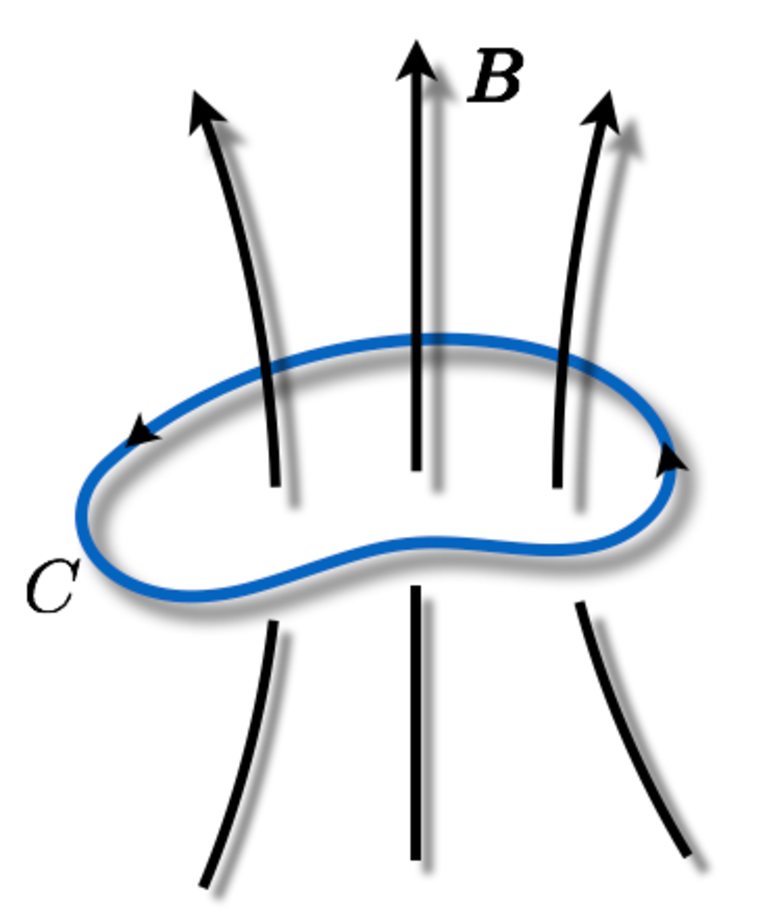
\includegraphics[width=0.25\textwidth]{Phi-a-traves-C}
	\caption{\emph{Flujo del campo $\B$ a través de un circuito cerrado $C$.}}\label{Phi-a-traves-C}
\end{figure}

La ley de Lenz es fundamental en el estudio de la energía electromagnética, es importante tener en cuenta que la ley de Lenz asegura que la transferencia de energía electromagnética se lleva a cabo de tal manera que se conserve la energía total del sistema, cumpliendo con el principio de conservación de la energía, ella establece que la dirección de la corriente inducida en un circuito cerrado $C$ es tal que se opone al cambio en el flujo magnético $\phi$ que la produce. Esto significa que la fem inducida $\xi_{ind}$ tendrá una polaridad que se opone al cambio en el flujo magnético.

	\begin{example}
		Una barra conductora de longitud $l$ que descansa sobre otro conductor doblado en forma de U de lados $l$ y $x$, si la barra se desplaza sobre el conductor a una velocidad constante $v$ y existe un campo magnetico $B$ el cual es normal al conductor. Calcular la fuerza electromotriz inducida.\\
		\emph{\textit{ Solución.}}\\

		La fem inducida viene dada por la ecuación~\eqref{Eq:Fza Electromotriz} de modo que,

		\begin{equation*}
			\xi_{ind} = -\diff{\phi}{t},
		\end{equation*}

		primero calculemos el flujo del campo magnético,

		\begin{equation*}
			\phi = \int_{S} \B \cdot \dl{\textbf{s}},
		\end{equation*}

		dado que el campo magnético $B$ es constante y normal a el area S, por lo que si consideramos que la barra se va desplazando, entonces el area S esta dado por, $S = lx$, de modo que,

		\begin{align*}
			\xi_{ind} &= -\diff*{\left( Blx \right) }{t},\\
								&= -Bl \diff{x}{t},\\
								&= -Blv.
		\end{align*}
	\end{example}

De la ecuación~\eqref{Eq:Fza Electromotriz} se puede observar que la fem inducida puede interpretarse como la presencia de un campo eléctrico inducido $\E_{ind}$ no conservativo a lo largo del alambre, de modo que podemos expresar~\eqref{Eq:LeyFaraday} como:

\begin{equation}
	\label{Eq:CampoETotal}
	\oint \E_{ind} \cdot \dl{\textbf{l}} = -\diff{\Phi}{t}.
\end{equation}

Para cualquier punto del espacio, el campo eléctrico total se puede expresar como la suma de una parte conservativa $\E_c$, y una parte no conservativa $\E_{ind}$, es decir $\E=\E_c+\E_{ind}$, de esta forma

\begin{equation*}
	\oint \E \cdot \dl{\textbf{l}} = \oint \E_{c} \cdot \dl{\textbf{l}} + \oint \E_{ind} \cdot \dl{\textbf{l}}.
\end{equation*}

De acuerdo con la ecuación~\eqref{Eq:CampoEConservativo} la primera integral del miembro derecho es cero debido a que se trata de un campo conservativo. Usando las ecuaciones~\eqref{Eq:FlujoMagnetico} y~\eqref{Eq:CampoETotal} podemos escribir:

\begin{equation}
	\label{Eq:FaradayVectoresCampo}
	\oint_{C} \E \cdot \dl{\textbf{l}} = -\diff*{ \int_{S} \B \cdot \dl{\textbf{s}} }{t}.
\end{equation}

La ecuación~\eqref{Eq:FaradayVectoresCampo}, representa las leyes de Faraday y Lenz expresadas en función de los campos y es valoda para cualquier trayectoria cerrada $C$ y por cuyalquier motivo por el cual el flujo de campo $\phi$ pueda cambiar. Debido a todas las formas en que este puede cambar, se estudiaran dos grandes categorias, si el medio esta en moviemnto o en reposo.

\subsection{Medios estacionarios}

Esta categoria aplica para todo sistema en el cual los medios conductores o circuitos de interes no se encuentran en movimento, por lo que las trayectorias cerradas $C$ no cambian de forma o tamaño, de manera que el flujo $\phi$ solo puede variar por que el campo $\B$ depende del tiempo, es decir, $\B = \B(\textbf{r}, t)$. Usando el teorema de Stokes en el miembro izquierdo de la ecuación~\eqref{Eq:FaradayVectoresCampo} obtenemos,

\begin{align*}
	\int_{S} \rotational{\E} \cdot \dl{\textbf{s}} &= -\diff*{ \int_{S} \B \cdot \dl{\textbf{s}} }{t},\\
	&= - \int_{S} \diffp{\B}{t} \cdot \dl{\textbf{s}}.
\end{align*}

Dado que esta expresión es valida para cualquier superficie $S$,

\begin{equation}
\label{Eq:LeyFaradayDiferencial}
	\rotational{\E} = -\diffp{\B}{t},
\end{equation}

esta expresión es conocida como la \emph{forma diferencial de la ley de Faraday}, y es la generalización de $\rotational{\E} = \textbf{0}$, que era valida para campos estáticos.

\begin{obs}
	Dado que de las ecuaciones~\eqref{Eq:Eq Electrostatica} la única que ha sido modificada es $\rotational{\E} = \textbf{0}$. Entonces sigue siendo valida la expresión $\divergence{\B} = \textbf{0}$, enonces podemos escribir,

	\begin{equation*}
		\B = \rotational{\textbf{A}}
	\end{equation*}

	Por lo tanto podemos reescribir a la ecuación~\eqref{Eq:LeyFaradayDiferencial} como,

	\begin{align*}
		\rotational{\E} &= -\diffp{\B}{t},\\
										&= -\diffp*{\left( \rotational{A} \right) }{t},\\
										&= \rotational{ \left(-\diffp{\textbf{A}}{t}\right) }.
	\end{align*}

	Si además se considera que para una función escalar $\phi$ siempre se satisface $\rotational{ \left( -\nabla \phi \right)} = \mathbf{0}$, entonces es posible escribir

	\begin{equation*}
		\rotational{\E} = \rotational{ \left( -\nabla\phi -\diffp{\textbf{A}}{t} \right)},
	\end{equation*}

	es decir,

	\begin{equation}
		\E = -\nabla\phi -\diffp{\textbf{A}}{t}.
	\end{equation}

	Lo que demuestra que en general el campo electrico $\E(\textbf{r}, t)$ depende del potencial escalar $\phi$ como del vectorial $\textbf{A}$.
\end{obs}
%
%
%
%
% Dado que ahora $\nabla\times\E\neq \textbf{0}$, es necesario estudiar las componentes tangenciales de $\E$ en una superficie de discontinuidad, para ello consideramos un peque\~no elemento de superficie en la capa de transición que sea perpendicular al flujo, tal como se ilustra en la figura (\ref{}), donde $\hat{\textbf{n}}\textbf{'}$ es el vector unitario normal a la superficie encerrada por la trayectoria $C$ y paralelo a la superficie entre $1$ y $2$, $\hat{\textbf{n}}$ es el vector unitario perpendicular a la  superficie, y el vector unitario $\hat{\textbf{t}}$ es paralelo al plano de $C$, de esta forma la integral de $\E$ alrededor de $C$ es
% \begin{equation}
% \oint_C\E\cdot \dl \textbf{l}&=&\E_2\cdot\hat{\textbf{t}}\,\,\Delta L-\E_1\cdot\hat{\textbf{t}}\,\,\Delta L+ \kappa\nonumber\\
% &=&\hat{\textbf{t}}\cdot\big(\E_2-\E_1\big)\,\Delta L+\kappa,\label{E en tra c}
% \end{equation}
% donde $\E_2$ y $\E_1$ son los valores de $\E$ en sus respectivas regiones, y $\kappa$ es la contribución a la integral de línea que resulta de los extremos de la trayectoria.
% Por otro lado, de la ec. (\ref{e to iq m part B}) se tiene que
% \begin{equation}
% \oint_C\E\cdot \dl \textbf{l}&=&-\int_S\frac{\partial\B}{\partial t}\cdot d\textbf{a}.
% \end{equation}
% De modo que
% \begin{equation}
% \oint_C\E\cdot \dl \textbf{l}&=&-\frac{\partial\B}{\partial t}\cdot\hat{\textbf{n}}\textbf{'}\,h\,\Delta L.\label{E constok i j}
% \end{equation}
% Igualando (\ref{E en tra c}) y (\ref{E constok i j}) obtenemos
% \begin{equation}
% \hat{\textbf{t}}\cdot\big(\E_2-\E_1\big)\,\Delta L+\kappa+\frac{\partial\B}{\partial t}\cdot\hat{\textbf{n}}'\,h\,\Delta L&=&0.
% \end{equation}
% Podemos observar de la figura que $\hat{\textbf{t}}=\hat{\textbf{n}}\times\hat{\textbf{n}}\textbf{'}$, entonces de la última expresión se tiene
% \begin{equation}
% (\hat{\textbf{n}}\times\hat{\textbf{n}}\textbf{'})\cdot\big(\E_2-\E_1\big)\,\Delta L+\frac{\partial\B}{\partial t}\cdot\hat{\textbf{n}}\textbf{'}\,h\,\Delta L&=&-\kappa.
% \end{equation}
% Para el primer término usamos la identidad
% \begin{equation}
% (\textbf{A}\times\B)\cdot\textbf{C}&=&(\textbf{C}\times\textbf{A})\cdot\B,
% \end{equation}
% así
% \begin{equation}
% -\kappa&=&\big[\big(\E_2-\E_1\big)\times\hat{\textbf{n}}\big]\cdot\hat{\textbf{n}}\textbf{'}\,\Delta L+\frac{\partial\B}{\partial t}\cdot\hat{\textbf{n}}\textbf{'}\,h\,\Delta L\nonumber\\
% &=&\left[ \big(\E_2-\E_1\big)\times\hat{\textbf{n}}+\frac{\partial\B}{\partial t}\,h\right] \cdot\hat{\textbf{n}}\textbf{'}\Delta L.
% \end{equation}
% Si ahora hacemos que $h\rightarrow 0$ entonces $\kappa\rightarrow 0$, de esta forma
% \begin{equation}
% \left[ \left( \E_2-\E_1\right) \times\hat{\textbf{n}}+\lim_{h\rightarrow 0}\left( \frac{\partial\B}{\partial t}\,h\right) \right] \cdot\hat{\textbf{n}}\textbf{'}\Delta L&=&0,
% \end{equation}
% Entonces
% \begin{equation}
% \big(\E_2-\E_1\big)\times\hat{\textbf{n}}&=&-\lim_{h\rightarrow 0}\left( \frac{\partial\B}{\partial t}\,h\right).\label{co f E tim}
% \end{equation}
% Podemos expresar $\E$ como la suma de sus componentes normales y transversales a la superficie de separación, es decir
% \begin{equation}
% \E&=&\E_n+\E_t\,\,\,=\,\,\,E_n\,\hat{\textbf{n}}+\E_t.\label{part trans y nor de e}
% \end{equation}
% Si realizamos el producto cruz con $\hat{\textbf{n}}$ en ambos miembros de (\ref{co f E tim})
% \begin{equation}
% \left[ \big(\E_{2}-\E_{1}\big)\times\hat{\textbf{n}}\right] \times\hat{\textbf{n}}&=&-\lim_{h\rightarrow 0}\left( h\frac{\partial\B}{\partial t}\times\hat{\textbf{n}}\right),\nonumber\\
% \big(\E_{2}-\E_{1}\big)(\hat{\textbf{n}}\cdot\hat{\textbf{n}})-\hat{\textbf{n}}\left[ \big(\E_{2}-\E_{1}\big)\cdot \hat{\textbf{n}}\right]&=&\textbf{0},\nonumber\\
% \big(\E_{2}-\E_{1}\big)-\hat{\textbf{n}}\big(E_{2}-E_{1}\big)&=&\textbf{0}.
% \end{equation}
% Usando la ec. (\ref{part trans y nor de e}) en esta última expresión
% \begin{equation}
% \E_{2t}-\E_{1t}&=&\textbf{0},\nonumber\\
% \Rightarrow\E_{2t}&=&\E_{1t}.
% \end{equation}
% Lo que demuestra que las componentes tangenciales del campo eléctrico son continuas.
%
%
%
% %*********************EJEMPLO********************
% \begin{example}
% Un conductor metálico que contiene forma de un segmento de alambre de longitud $l$ se mueve en un campo $\B$ con velocidad $\textbf{v}$ (figura \ref{alambre-mov-en-B}). Partiendo de una consideración detallada de la fuerza de Lorentz sobre los electrones en el alambre, demuestre que los extremos de este están a la diferencia de potencial $\B\cdot\textbf{l}\times\textbf{v}$.\\
% \begin{figure}[H]
%   \centering
%     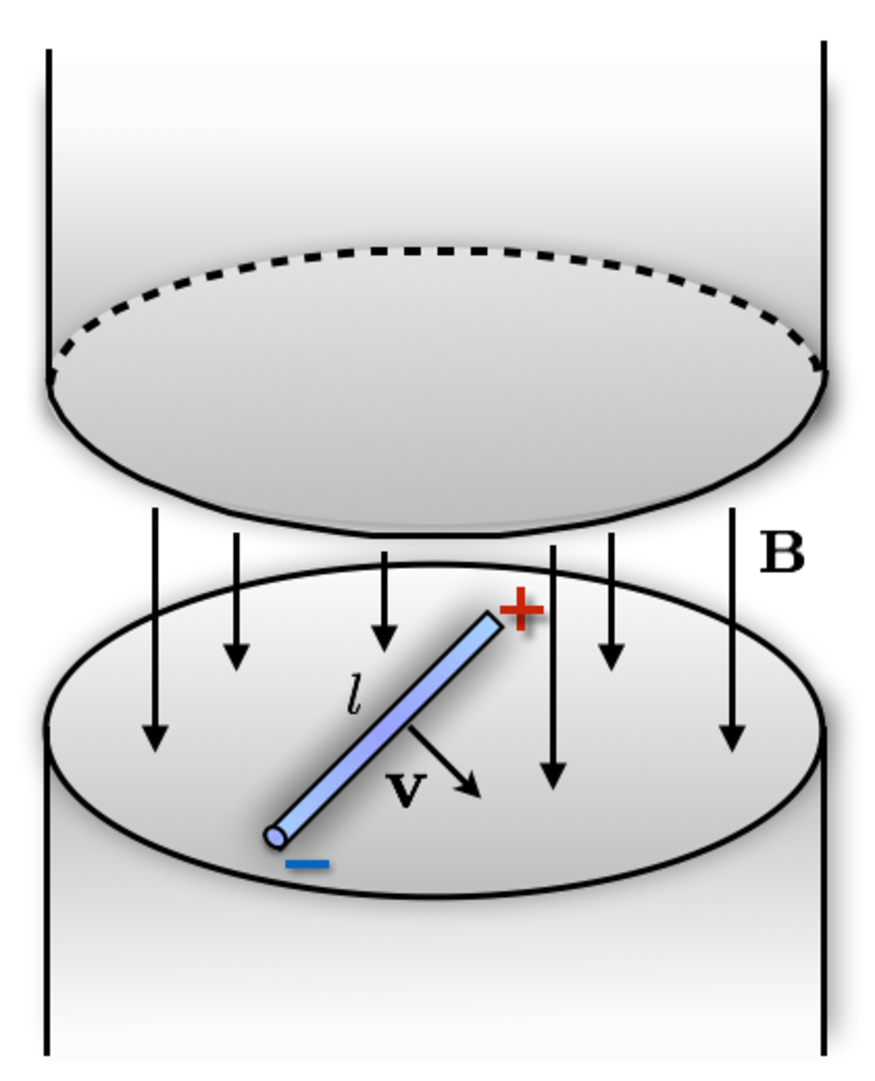
\includegraphics[width=0.25\textwidth]{alambre-mov-en-B}
%         \caption{\emph{Potencial eléctrico producido por movimiento de segmento de alambre en un campo $\B$.}}\label{alambre-mov-en-B}
% \end{figure}\\
% \emph{Solución.}\\
% Las cargas libres del conductor experimentan una fuerza de Lorentz que conduce a las cargas positivas y negativas a los extremos del alambre
% \begin{equation}
% \textbf{F}&=&q(\E+\textbf{v}\times\B),\nonumber\\
% m\textbf{a}&=&q(\E+\textbf{v}\times\B).
% \end{equation}
% Cuando las cargas no se mueven con respecto al alambre, la fuerza total sobre cada carga es cero, de modo que
% \begin{equation}
% \E&=&-\textbf{v}\times\B.\label{fz d lor en alambr en cmp b}
% \end{equation}
% Por otro lado, recordamos que la diferencia de potencial se puede calcular como
% \begin{equation}
% \Delta\phi&=&-\int\E\cdot \dl \textbf{l}.%,\nonumber\\
% %&=&-\E\cdot\textbf{l}.
% \end{equation}
% Así, de la ec. (\ref{fz d lor en alambr en cmp b}) se tiene que
% \begin{equation}
% \Delta\phi&=&(\textbf{v}\times\B)\cdot\textbf{l},\nonumber\\
% &=&-(\B\times\textbf{v})\cdot\textbf{l}.
% \end{equation}
% Usando la identidad
% \begin{equation}
% (\textbf{A}\times\B)\cdot\textbf{C}&=&\textbf{A}\cdot(\B\times\textbf{C}).\nonumber\\
% &=&-\textbf{A}\cdot(\textbf{C}\times\B).
% \end{equation}
% Entonces
% \begin{equation}
% \therefore\Delta\phi&=&\B\cdot(\textbf{l}\times\textbf{v}).
% \end{equation}
% \end{example}
%
%
%
% %*********************EJEMPLO********************
% \begin{example}
% Una varilla metálica de longitud $l$ gira en torno a un eje, que pasa por uno de sus extremos y es perpendicular a la varilla, con una velocidad angular $\omega$. El plano de rotación de la varilla es perpendicular a un campo de inducción magnética $\B$ (figura \ref{varilla-girando-en-B}). ?`Cual es la fem de movimiento inducido entre los extremos de la varilla?.\\
% \begin{figure}[H]
%   \centering
%     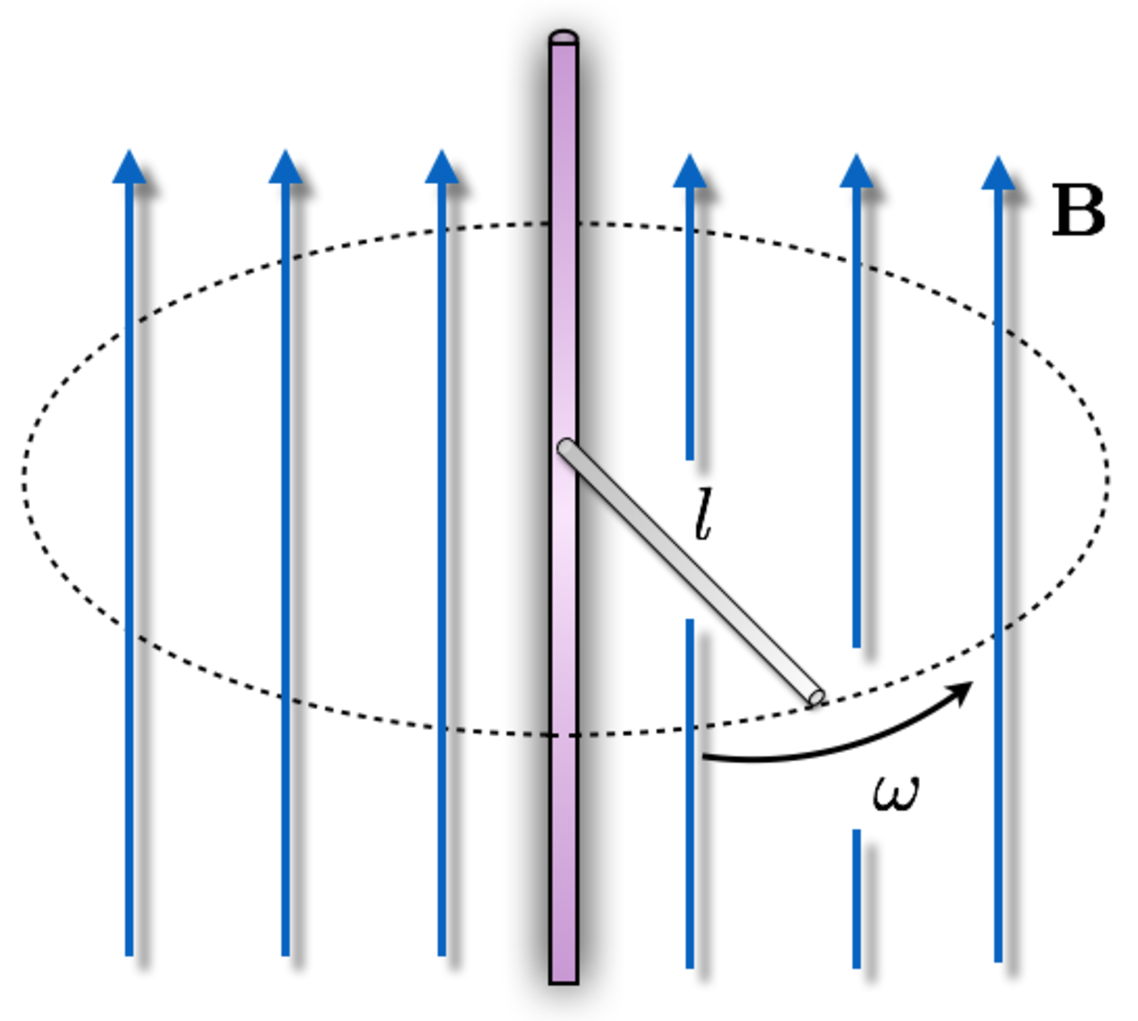
\includegraphics[width=0.3\textwidth]{varilla-girando-en-B}
%         \caption{\emph{Varilla girando con una velocidad angular $\omega$ perpendicular a un campo de inducción magnética $\B$.}}\label{varilla-girando-en-B}
% \end{figure}\\
% \emph{Solución.}\\
% Al igual que en el problema anterior, las cargas libres del conductor experimentan una fuerza de Lorentz que conduce a las cargas positivas y negativas a los extremos del alambre
% \begin{equation}
% \textbf{F}&=&q(\E+\textbf{v}\times\B),\nonumber
% \end{equation}
% En el caso estacionario la fuerza total sobre cada carga es cero, con lo que
% \begin{equation}
% \E&=&-\textbf{v}\times\B.
% \end{equation}
% Como $\textbf{v}\perp\B$ entonces
% \begin{equation}
% E&=&\mbox{v}B,\nonumber\\
% &=&\omega lB\,\,\,\,,\,\,\,\,\mbox{con}\,\,\,\,\mbox{v}=\omega l.\label{e cn v perp b y vwl}
% \end{equation}
% Por otro lado, de la ec. (\ref{ley de faraday}) sabemos que
% \begin{equation*}
% \xi_{ind}&=&-\frac{d\Phi}{dt}.
% \end{equation*}
% Pero sabemos también que la  fem inducida puede interpretarse como la presencia de un campo eléctrico inducido $\E_{ind}$ no conservativo a lo largo del alambre, de modo que
% \begin{equation}
% \xi_{ind}&=&\int\E_{ind}\cdot \dl \textbf{l}.
% \end{equation}
% Usando la ec. (\ref{E tot iq Ec + Eind}) y despues (\ref{e cn v perp b y vwl}) se obtiene
% \begin{equation}
% \xi_{ind}&=&\int_0^l\E\cdot \dl \textbf{l}.\nonumber\\
% &=&\int_0^l \omega lB\,\,dl,\nonumber\\
% \therefore\xi_{ind}&=&\omega B\,\frac{l^2}{2}.
% \end{equation}
% \end{example}
%
%
% %*********************EJEMPLO********************
% \begin{example}
% El generador homopolar de Faraday consiste en un disco de metal que gira en un campo magnético uniforme que es perpendicular a su plano (figura \ref{generador-homopolar-de-Faraday}). Demuestre que la diferencia de potencial que se genera entre el centro y la periferia del disco es $\xi=f\,\Phi$, donde $\Phi$ es el flujo que atraviesa el disco y $f$ es la frecuencia con la que gira.\\
% \begin{figure}[H]
%   \centering
%     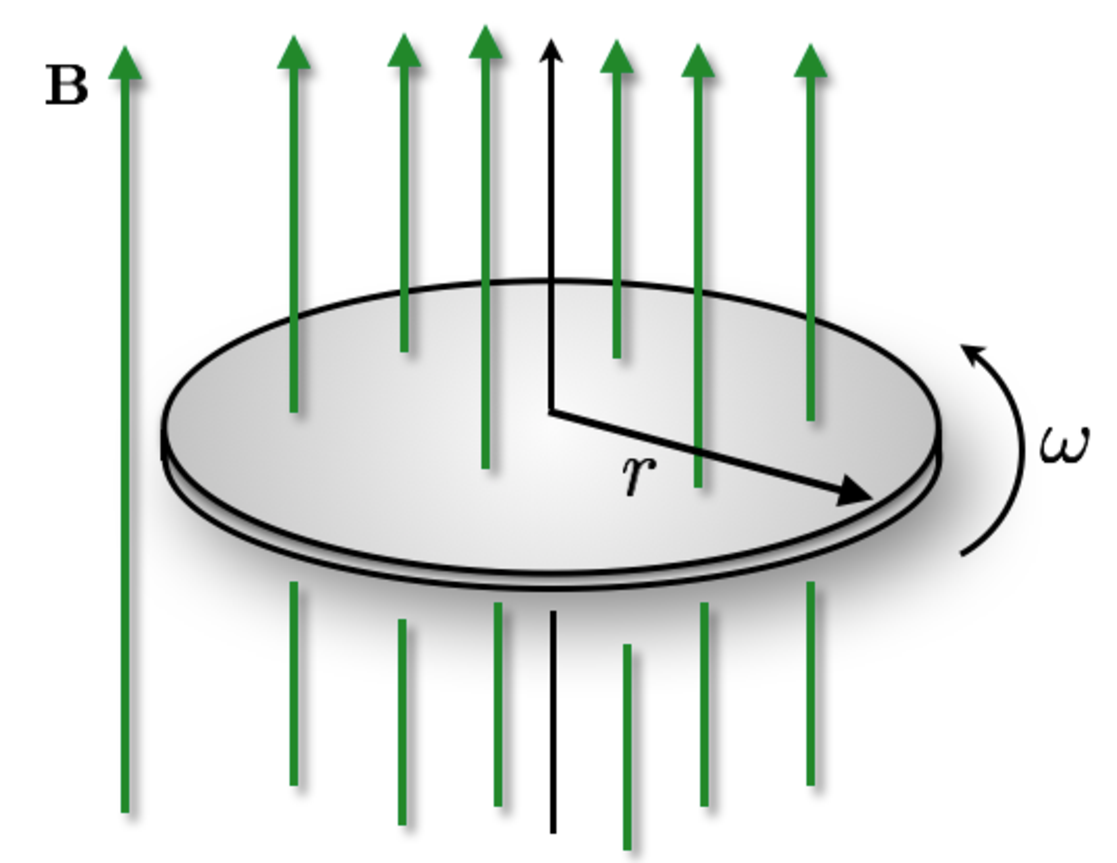
\includegraphics[width=0.35\textwidth]{generador-homopolar-de-Faraday}
%         \caption{\emph{Generador homopolar de Faraday.}}\label{generador-homopolar-de-Faraday}
% \end{figure}\\
% \emph{Solución.}\\
% Sabemos que
% \begin{equation*}
% \xi_{ind}&=&\int\E\cdot \dl \textbf{l},
% \end{equation*}
% En el caso estacionario, de la fuerza de Lorentz se tiene
% \begin{equation}
% \E&=&-\textbf{v}\times\B,\nonumber\\
% \Rightarrow E&=&\mbox{v}B,\nonumber\\
% &=&\omega rB,\nonumber\\
% &=&2\pi\,f\,r\,B.
% \end{equation}
% Donde se usó $\mbox{v}=\omega r=2\pi\,fr$. Con esto se tiene que
% \begin{equation}
% \xi_{ind}&=&\int 2\pi\,frB\,\,dr,\nonumber\\
% &=&\pi\,fBr^2.\label{xi en disc}
% \end{equation}
% Por otro lado recordamos que el flujo magnético está dado por
% \begin{equation}
% \Phi&=&\int \B\cdot \dl \textbf{a},\nonumber\\
% &=&B\pi r^2.
% \end{equation}
% Sustituyendo esta última expreción en (\ref{xi en disc}) se obtiene finalmente que
% \begin{equation}
% \therefore\xi_{ind}&=&f\,\Phi.
% \end{equation}
% \end{example}
%
%
%
%
% %*********************EJEMPLO********************
% \begin{example}
% Un cilindro dieléctrico de permitividad $\varepsilon$ gira entorno a su eje con una velocidad $\omega$. Si existe un campo magnético uniforme $\B$ paralelo al eje del cilindro, halle la carga de polarización inducida en el dieléctrico.\\
% \begin{figure}[H]
%   \centering
%     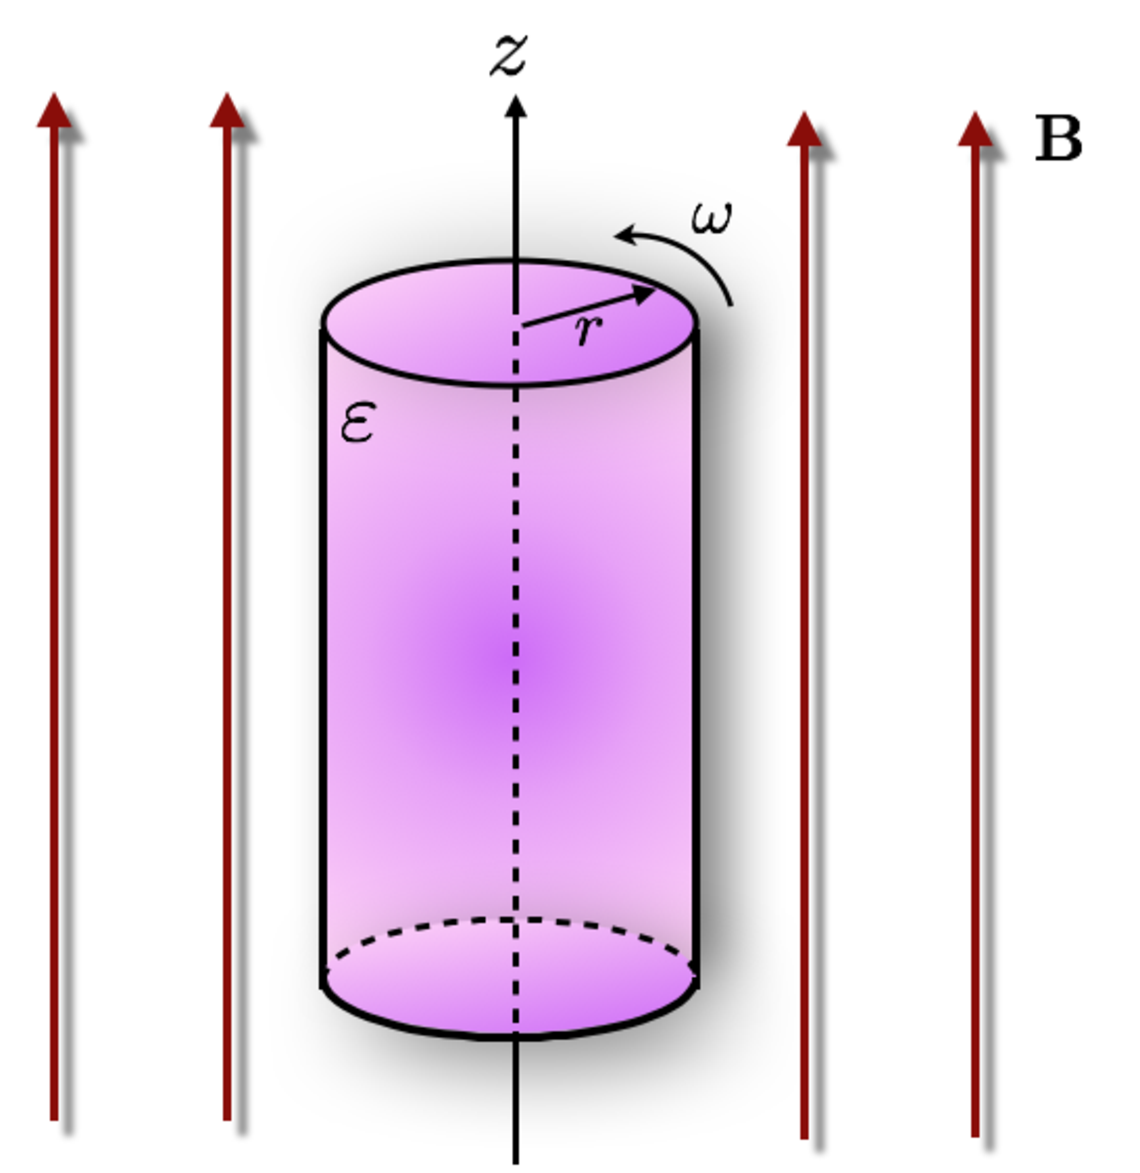
\includegraphics[width=0.35\textwidth]{Cilindro-dielectrico-girando-en-campo-B}
%         \caption{\emph{Cilindro dieléctrico giratorio, inmerso en campo $\B$.}}\label{Cilindro-dielectrico-girando-en-campo-B}
% \end{figure}\\
% \emph{Solución.}\\
% Supongamos que el eje del cilindro se orienta paralelo al eje $z$ (figura \ref{Cilindro-dielectrico-girando-en-campo-B}). Las cargas del dieléctrico experimentan una fuerza de Lorentz que las alinea de forma radial al eje del cilindro
% \begin{equation*}
% \textbf{F}&=&q(\E+\textbf{v}\times\B).
% \end{equation*}
% Cuando las cargas no se mueven con respecto al cilindro, la fuerza total sobre cada carga es cero, de modo que
% \begin{equation}
% \E&=&-\textbf{v}\times\B,
% \end{equation}
% donde
% \begin{equation}
% \textbf{v}&=& r\omega\,\hat{\pmb{\varphi}}.\\
% \B&=&B\,\hat{\textbf{k}}.
% \end{equation}
% Entonces
% \begin{equation}
% \E&=&-r\omega B (\hat{\pmb{\varphi}}\times\hat{\textbf{k}}),\nonumber\\
% &=&-r\omega B\,\hat{\pmb {r}}.
% \end{equation}
% Por otro lado, recordamos que la polarización se puede obtener como
% \begin{equation}
% \textbf{P}&=&\chi\E,\nonumber\\
% &=&-\chi r\omega B\,\hat{\pmb {r}},\nonumber\\
% &=&(\varepsilon_0-\varepsilon) r\omega B\,\hat{\pmb {r}}\,\,\,\,\,\,\,;\,\,\,\,\,\,\,con\,\,\,\,\,\,\,\,\chi=\varepsilon-\varepsilon_0.
% \end{equation}
% De la ec. (\ref{carga de polarizacion}) se tiene que la carga de polarización está dada como
% \begin{equation}
% Q_p&=&\oint_S\textbf{P}\cdot\hat{\textbf{n}}\,\,da\textbf{'}-\int_V\nabla\cdot\textbf{P}\,\,d\mbox{v}\textbf{'},\nonumber\\
% &=&(\varepsilon_0-\varepsilon)\omega B\int_{0}^{L}\int_{0}^{r}\,\,r\textbf{'}^2dr\textbf{'}dz\textbf{'}-(\varepsilon_0-\varepsilon)\omega B\int_{0}^{L}\int_{0}^{2\pi}\int_{0}^{r}\frac{1}{r\textbf{'}}\frac{\partial r\textbf{'}^2}{\partial r\textbf{'}}\,r\textbf{'}dr\textbf{'}\,d\varphi\textbf{'}dz\textbf{'},\nonumber\\
% &=&(\varepsilon_0-\varepsilon)\omega B\left(\frac{L\,r^3}{3}-2\pi \,L\,r^2 \right), \nonumber\\
% \nonumber\\
% \therefore Q_p&=&(\varepsilon_0-\varepsilon)\omega B\,L\,r^2\left(\frac{r}{3}-2\pi\right).
% \end{equation}
% \end{example}
%
%
%
%
% %*********************SECCION********************
% \section{Inductancia. Inductancia mutua}
% Consideremos dos circuitos filamentales $C_1$ y $C_2$, con las corrientes $I_1$ e $I_2$ respectivamente (figura \ref{fig6.1}). La corriente $I_2$ producirá una inducción $\B_2$ en cada punto de la superficie $S_1$ encerrada por $C_1$, por lo que es posible calcular el flujo $\Phi_{2\rightarrow 1}$ en $C_1$ por medio de (\ref{flujo madnetico})
% \begin{equation}
% \Phi_{2\rightarrow 1}&=&\int_{S_1}\B_2(\textbf{r}_1)\cdot \dl \textbf{a}_1.
% \end{equation}
% \begin{figure}[H]
%   \centering
%     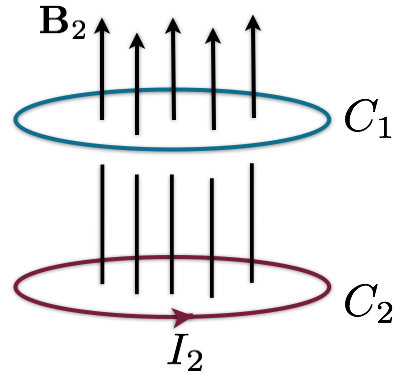
\includegraphics[width=0.3\textwidth]{Induc}
%         \caption{\emph{Inducción magnética.}}\label{fig6.1}
% \end{figure}
% Sustituyendo la ec. (\ref{rot A})
% \begin{equation}
% \Phi_{2\rightarrow 1}&=&\int_{S_1}\left[ \nabla\times\textbf{A}_2(\textbf{r}_1)\right] \cdot \dl \textbf{a}_1,
% \end{equation}
% usando el teorema de Stokes
% \begin{equation}
% \Phi_{2\rightarrow 1}&=&\oint_{C_1} \textbf{A}_2(\textbf{r}_1)\cdot \dl \textbf{l}_1.
% \end{equation}
% Ahora sustituimos la ec. (\ref{potencial magnetico filamental})
% \begin{equation}
% \Phi_{2\rightarrow 1}=\frac{\mu_0}{4\pi}\oint_{C_1}\oint_{C_2}\frac{I_2\,\dl \textbf{l}_1\cdot d\textbf{l}_2}{R_{12}},\label{fluj pji 2-1}
% \end{equation}
% definimos la \emph{inductancia mutua} de los circuitos $1$ y $2$ como
% \begin{equation}
% M_{12}= \frac{\mu_0}{4\pi}\oint_{C_1}\oint_{C_2}\frac{\dl \textbf{l}_1\cdot d\textbf{l}_2}{R_{12}}.
% \end{equation}
% En general para dos circuitos $C_i$ y $C_j$
% \begin{equation}
% M_{ij}= \frac{\mu_0}{4\pi}\oint_{C_i}\oint_{C_j}\frac{\dl \textbf{l}_i\cdot d\textbf{l}_j}{R_{ij}},\label{inductancia mutua}
% \end{equation}
% de esta forma el flujo a través de $C_i$ debido a $C_j$ será
% \begin{equation}
% \Phi_{j\rightarrow i}&=&M_{ij}\,I_j.\label{flujo marn en term de M}
% \end{equation}
% Podemos observar de (\ref{inductancia mutua}) que la inductancia mutua es un factor puramente geométrico que relaciona los tama\~nos y orientaciones de los circuitos. Dado que las unidades de $\mu_0$ son henry/metro, entonces la unidad de la inductancia mutua es el henry.\\
% \\
% De manera análoga, si se calcula el flujo en $C_j$ debido a $C_i$ se encuentra que
% \begin{equation}
% M_{ji}&=& \frac{\mu_0}{4\pi}\oint_{C_j}\oint_{C_i}\frac{\dl \textbf{l}_j\cdot d\textbf{l}_i}{R_{ji}},\label{Mji}\\
% \Phi_{i\rightarrow j}&=&M_{ji}\,I_i.
% \end{equation}
% Es evidente que
% \begin{equation}
% M_{ij}=M_{ji}.
% \end{equation}
% La fem total inducida que producirá uno de los circuitos por una corriente cambiante en el otro, puede expresarse en función de  la inductancia mutua sustituyendo (\ref{flujo marn en term de M})  en (\ref{ley de faraday})
% \begin{equation}
% \xi_{j\rightarrow i}=-\,M_{ij}\,\frac{dI_j}{dt}.
% \end{equation}
% Si existe mas de un circuito produciendo un campo $\B$ a través de $C_i$, el flujo total será una suma de términos como (\ref{flujo marn en term de M})
% \begin{equation}
% \Phi_i=\sum_j\Phi_{j\rightarrow i}\,\,\,=\,\,\,\sum_jM_{ij}\,I_j.\label{fluj tot en Ci}
% \end{equation}
% De manera que la fem total inducida en $C_i$ por los otros circuitos será
% \begin{equation}
% \xi_{i}&=&-\,\sum_jM_{ij}\,\frac{dI_j}{dt}.\label{fem ind C_i}
% \end{equation}
%
% Para encontrar una expresión mas detallada de (\ref{Mji}) se usa la figura \ref{Induct}, de la cual se deduce
% \begin{equation}
% R=\sqrt{d^2_{ij}+r^2},\ \ \ r=\sqrt{r^2_i+r^2_j-2\ r_i\ r_j \cos \theta},
% \end{equation}
% además
% \begin{equation}
% \dl \textbf{l}_i\cdot d\textbf{l}_j=dl_i\ dl_j \cos \theta\,\,\, \mbox{y}\,\, \,    dl_i=r_i\ d\theta.
% \end{equation}
%
% \begin{figure}[H]
% \centering
% 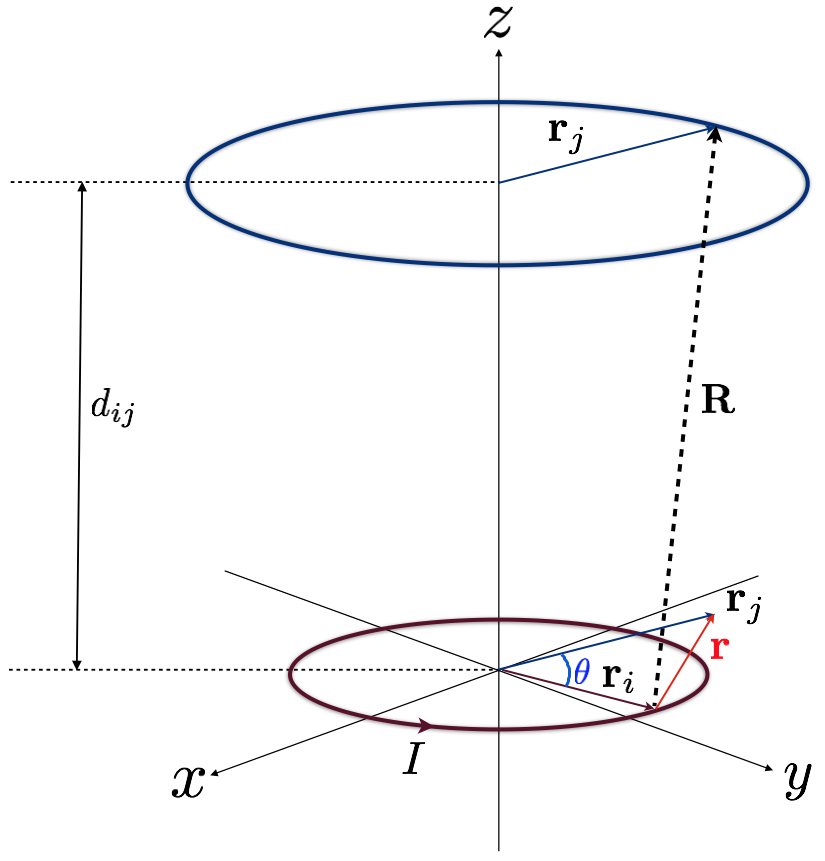
\includegraphics[scale=.25]{Induc1}
% 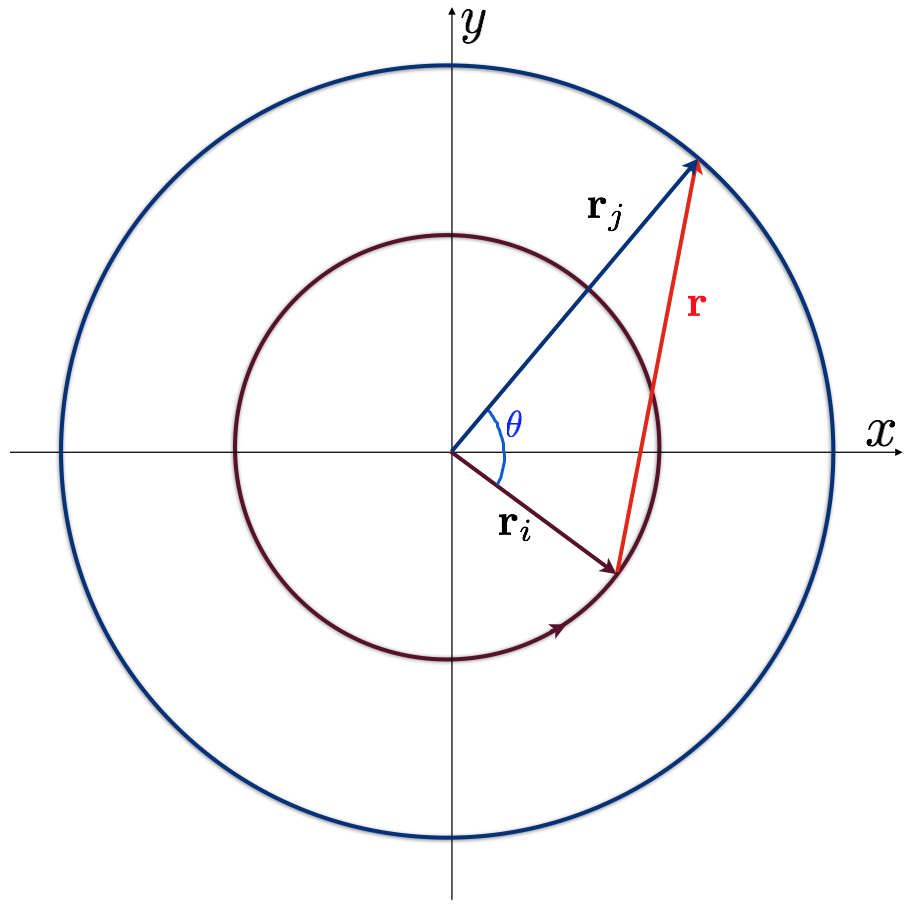
\includegraphics[scale=.2]{Induc2}
% \caption{{\it Dos lazos conductores de radios $r_j$ y $r_i$.}} \label{Induct}
% \end{figure}
% Así se tiene
% \begin{equation}
% M_{ij}&=&\dfrac{\mu_0}{4\pi}\oint \int^{2\pi}_0\dfrac{r_i\ \cos \theta\, d\theta\ dl_j}{\sqrt{d^2_{ij}+r^2_i+r^2_j-2\ r_i\ r_j \cos \theta}},
% \end{equation}
% para continuar se hace el cambio de variable $\theta=2\alpha$, así que
% \begin{equation}
% M_{ij}&=&\dfrac{\mu_0}{4\pi} r_i (2\pi r_j)\int^{\pi}_0\dfrac{\cos (2\alpha)\, 2d\alpha}{\sqrt{d^2_{ij}+r^2_i+r^2_j-2\ r_i\ r_j \cos (2\alpha)}},\nonumber\\
% &=&\mu_0 r_i\ r_j\int^{\pi}_0\dfrac{\cos (2\alpha)\, d\alpha}{\sqrt{d^2_{ij}+r^2_i+r^2_j-2\ r_i\ r_j \cos (2\alpha)}}.
% \end{equation}
% Dado que $\cos (2\alpha)=1-2\sen^2\alpha$ entonces
% \begin{equation}
% M_{ij}&=&\mu_0\ r_i\ r_j\int^{\pi}_0\dfrac{(1-2\sin^2 \alpha)\, d\alpha}{\sqrt{d^2_{ij}+(r_i-r_j)^2+4\ r_i\ r_j \sin^2 \alpha}},
% \end{equation}
% ahora se emplea
% \begin{equation}
% \sin^2\alpha+\cos^2\alpha=1, \label{iTrig}
% \end{equation}
% por lo cual
% \begin{equation}
% d^2_{ij}+(r_i-r_j)^2+4\ r_i\ r_j \sin^2 \alpha&=&\big(d^2_{ij}+(r_i-r_j)^2 \big)(\cos^2\alpha+\sin^2\alpha)+4\ r_i\ r_j \sin^2 \alpha,\nonumber\\
% &=&\Big(d^2_{ij}+(r_i-r_j)^2 \Big) \cos^2\alpha+\Big(d^2_{ij}+(r_i+r_j)^2 \Big) \sin^2 \alpha ,\nonumber\\
% &=&\Big(d^2_{ij}+(r_i-r_j)^2 \Big) \left[ \cos^2\alpha+\frac{d^2_{ij}+(r_i+r_j)^2}{d^2_{ij}+(r_i-r_j)^2}\sin^2 \alpha\right]  ,\nonumber\\
% &=&\Big(d^2_{ij}+(r_i-r_j)^2 \Big) \left[ \cos^2\alpha+k^2_c \sin^2 \alpha \right],
% \end{equation}
% con
% \begin{equation}
% k^2_c:=\frac{d^2_{ij}+(r_i+r_j)^2}{d^2_{ij}+(r_i-r_j)^2}.
% \end{equation}
% Al usar estas expresiones en el cáculo para $M_{ij}$ se tiene
% \begin{equation}
% M_{ij}&=&\frac{\mu_0\ r_i\ r_j}{\sqrt{d^2_{ij}+(r_i-r_j)^2}} \int^{\pi}_0\dfrac{(1-2\sin^2 \alpha)\, d\alpha}{\sqrt{\cos^2\alpha+k^2_c \sin^2 \alpha}},\nonumber\\
% &=&\frac{\mu_0\ r_i\ r_j}{\sqrt{d^2_{ij}+(r_i-r_j)^2}}\left( \int^{\pi}_0\dfrac{d\alpha}{\sqrt{\cos^2\alpha+k^2_c \sin^2 \alpha}}-2\int^{\pi}_0\dfrac{\sin^2 \alpha\ d\alpha}{\sqrt{\cos^2\alpha+k^2_c \sin^2 \alpha}}\right),\nonumber\\
% \end{equation}
% nuevamente se usa (\ref{iTrig}) para simplificar un poco esta última expresión (con $a^2:=k^2_c-1$)
% \begin{equation}
% M_{ij}&=&\frac{\mu_0\ r_i\ r_j}{\sqrt{d^2_{ij}+(r_i-r_j)^2}}\left( \int^{\pi}_0\dfrac{d\alpha}{\sqrt{1+a^2 \sin^2 \alpha}}-2\int^{\pi}_0\dfrac{\sin^2 \alpha\ d\alpha}{\sqrt{1+a^2 \sin^2 \alpha}}\right).
% \end{equation}
% Dada la simetría del integrando se puede hacer un cambio en los límites de integración, de tal forma que se tiene
% \begin{equation}
% M_{ij}&=&\frac{2\mu_0\ r_i\ r_j}{\sqrt{d^2_{ij}+(r_i-r_j)^2}}\left( \int^{\pi/2}_0\dfrac{d\alpha}{\sqrt{1+a^2 \sin^2 \alpha}}-2\int^{\pi/2}_0\dfrac{\sin^2 \alpha\ d\alpha}{\sqrt{1+a^2 \sin^2 \alpha}}\right),\, \, \, \, \label{IntElip}
% \end{equation}
% este resultado se puede  escribir de la forma (Ver Apéndice \ref{Integrales})
% \begin{equation}
% M_{ij}&=&\mu_0 \sqrt{r_ir_j}\dfrac{2}{k}\left[\left(1 -\frac{k^2}{2}\right) F[k,\pi/2]-E[k,\pi/2]\right],%COINCIDE CON INDUCT2.PDF
% \end{equation}
% con $k^2:=\frac{a^2}{1+a^2}$. Estas integrales elípticas, $F[k,\pi/2]$ y $E[k,\pi/2]$ no se pueden resolver analíticamente por lo cual se resuelven numéricamente. Por ejemplo usando  {\it MATHEMATICA 9.0.1}  se tiene
% \begin{equation}
% &&\mbox{EllipticeF}[\pi/2,0.4]=1.77752,\\
% &&\mbox{EllipticeE}[\pi/2,0.4]=1.39939\, .
% \end{equation}
%
% %%%%%%%%%%%%%%%%%%%%SECCION%%%%%%%%%%%%%
% \section{Autoinductancia}
% Es posible que el circuito $C_i$ produzca un flujo $\Phi_{i\rightarrow i}$ que pase a través de sí mismo (figura \ref{Bt}). El coeficiente de proporcionalidad en este caso se denomina \emph{autoinductancia}. Entonces de la ec. (\ref{fluj pji 2-1})
% \begin{equation}
% \Phi_{i\rightarrow i}&=& \frac{\mu_0}{4\pi}\oint_{C_i}\oint_{C_i}\frac{I_i\,\dl \textbf{l}_i\cdot d\textbf{l}_i'}{R_{ii}}.
% \end{equation}
% \begin{figure}[H]
%   \centering
%     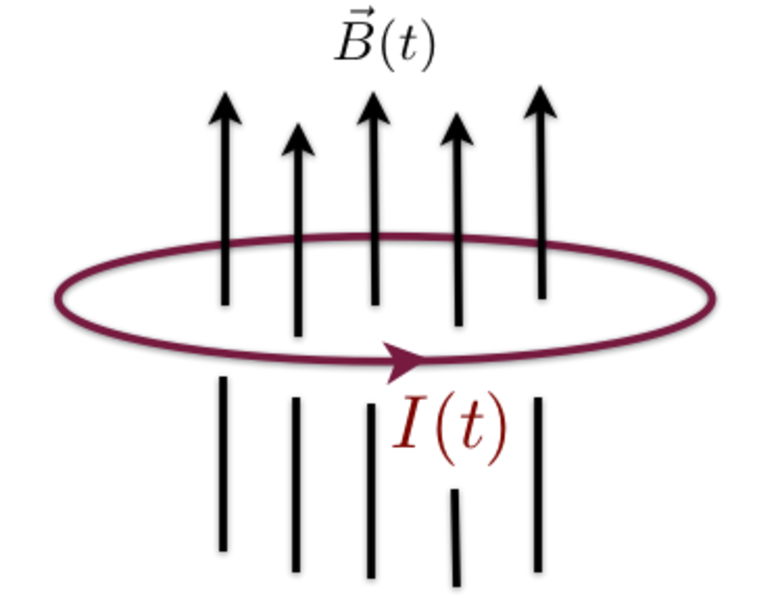
\includegraphics[width=0.4\textwidth]{AutoIn}
%         \caption{Autoinductancia.}\label{Bt}
% \end{figure}
%
% Así
% \begin{equation}
% L_{ii}&=& \frac{\mu_0}{4\pi}\oint_{C_i}\oint_{C_i}\frac{\dl \textbf{l}_i\cdot d\textbf{l}_i'}{R_{ii}},\\
% \Rightarrow\Phi_{i\rightarrow i}&=&L_{ii}I_i.\label{fluj de Ci en Ci}
% \end{equation}
% La doble integral se toma dos veces sobre el mismo circuito, y d$\textbf{l}$ y d$\textbf{l'}$ son dos elementos lineales pertenecientes a $C_i$. Si la corriente $I_i$ está cambiando existirá una fem inducida debido a su propio flujo, denominada \emph{fem autoinducida} o \emph{contra fem} y está dada por
% \begin{equation}
% \xi_i &=&-\,L_{ii}\,\frac{dI_i}{dt}.\label{fem aut ind}
% \end{equation}
% A menudo se suprimen uno o más de los índices de la autoinductancia siempre que esto no cause confusión.\\
% \\
% Si existen otros circuitos en las cercanías, el flujo total en $C_i$ será la suma de (\ref{fluj tot en Ci}) y (\ref{fluj de Ci en Ci})
% \begin{equation}
% \Phi_i&=&\sum_jM_{ij}\,I_j+L_{ii}I_i,\nonumber\\
% \Phi_i&=&\sum_jM_{ij}\,I_j\,\,\,\,\,\,con\,\,\,\,\,\,\,M_{ii}=L_{ii}.\label{fluj tot en Ci inclu C_i}
% \end{equation}
% El índice $i$ toma el valor de $j$. Por otro lado la fem total inducida será la suma de (\ref{fem ind C_i}) y (\ref{fem aut ind})
% \begin{equation}
% \xi_i&=&-\,\sum_jM_{ij}\,\frac{dI_j}{dt}-L_{ii}\,\frac{dI_i}{dt},\nonumber\\
% \xi_i&=&-\,\sum_jM_{ij}\,\frac{dI_j}{dt}.\label{fem tot ind en C_i}
% \end{equation}
%
%
%
%
%
% %*********************EJEMPLO********************
% \begin{example}
% Un circuito está formado por dos cáscaras cilíndricas coaxiales de radios $R_1$ y $R_2$ ($R_2>R_1$) y de longitud común $L$, conectados por placas  de extremos planos. La carga fluye hacia una cáscara y regresa  a la otra (figura \ref{cascaras-cilindricas-coaxiales-con-corriente}). ?`Cuál es la autoinductancia de este circuito?.\\
% \begin{figure}[H]
%   \centering
%     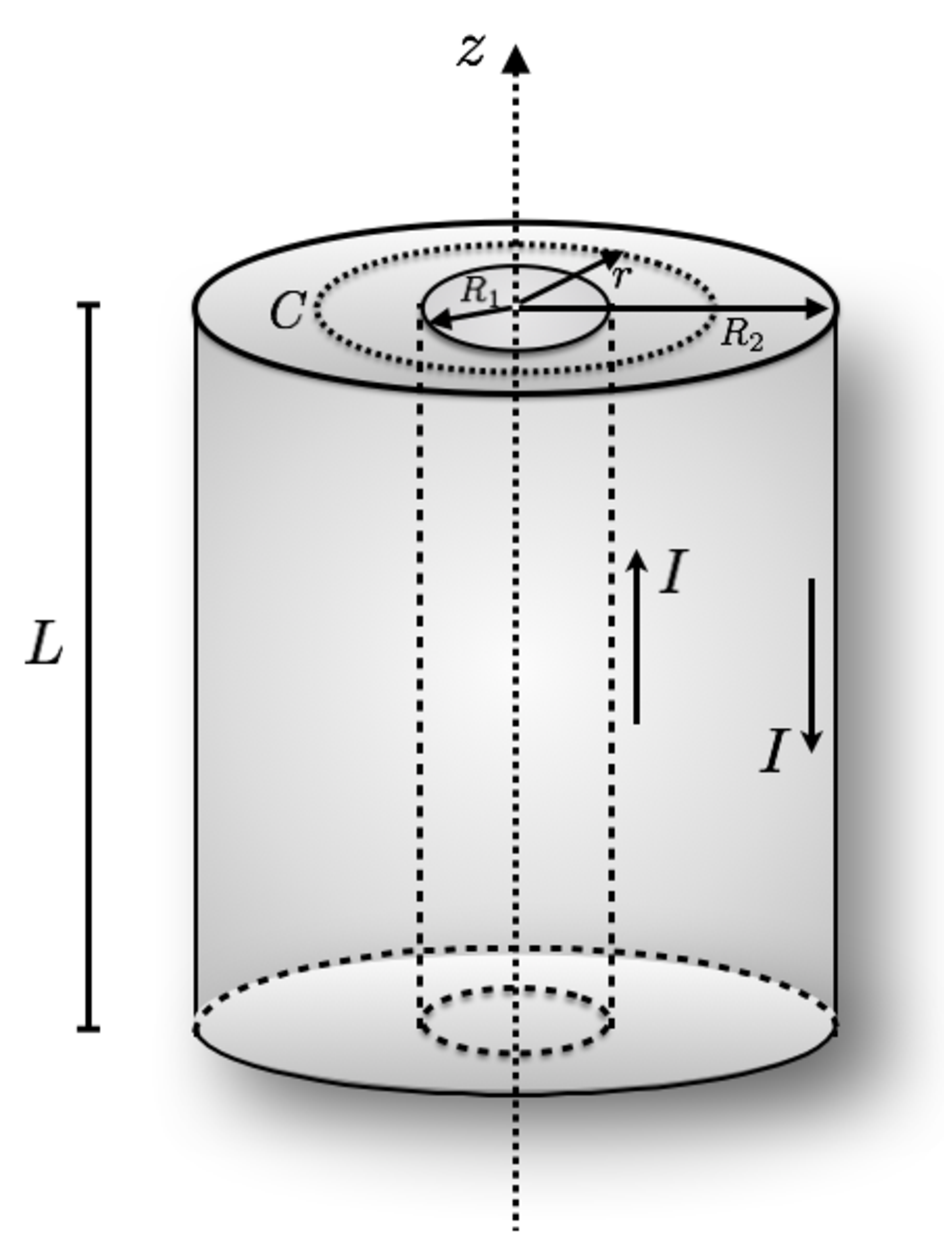
\includegraphics[width=0.35\textwidth]{cascaras-cilindricas-coaxiales-con-corriente}
%         \caption{\emph{Cáscaras cilíndricas coaxiales de longitud $L$.}}\label{cascaras-cilindricas-coaxiales-con-corriente}
% \end{figure}\\
% \emph{Solución.}\\
% Supongamos que las cáscaras cilíndricas se orientan paralelas al eje $z$. De la ec. (\ref{fluj de Ci en Ci}) se obtiene
% \begin{equation}
% d\Phi&=&L\,dI,\nonumber\\
% \Rightarrow L&=&\frac{d \Phi}{dI}.
% \end{equation}
% Donde $\Phi$ está dado por
% \begin{equation*}
% \Phi&=&\int_S\B\cdot \dl \textbf{a}.
% \end{equation*}
% Por otro lado, recordamos de la ley de Ampere que
% \begin{equation*}
% \oint_C\B\cdot \dl \textbf{l}&=&\mu_0\,I_{enc}.
% \end{equation*}
% Consideremos una curva de radio $R_1<r<R_2$, así
% \begin{equation}
% \int_0^{2\pi}\B\cdot \dl \textbf{l}&=&\mu_0\,I,\nonumber\\
% B&=&\frac{\mu_0\, I}{2\pi\,r},\nonumber\\
% \Rightarrow\B&=&\frac{\mu_0\, I}{2\pi\,r}\,\hat{\pmb{\varphi}}.
% \end{equation}
% Con lo que
% \begin{equation}
% \Phi&=&\frac{\mu_0\, I}{2\pi}\int_{R_1}^{R_2}\int_{0}^{L} \frac{1}{r}\,\,dz\,dr,\nonumber\\
% &=&\frac{\mu_0\, I\, L}{2\pi}\ln\left( \frac{R_2}{R_1}\right).
% \end{equation}
% De esta forma
% \begin{equation}
% L&=&\frac{\mu_0\, L}{2\pi}\ln\left( \frac{R_2}{R_1}\right)\frac{d\,I}{dI},\nonumber\\
% \therefore L&=&\frac{\mu_0\, L}{2\pi}\ln\left( \frac{R_2}{R_1}\right).
% \end{equation}
% \end{example}
%
%
% %%%%%%%%%%%%%%%%EJEMPLO%%%%%%%%%
% \begin{example}Circuito R-L.
%
% \begin{figure}[ht]
%   \centering
%     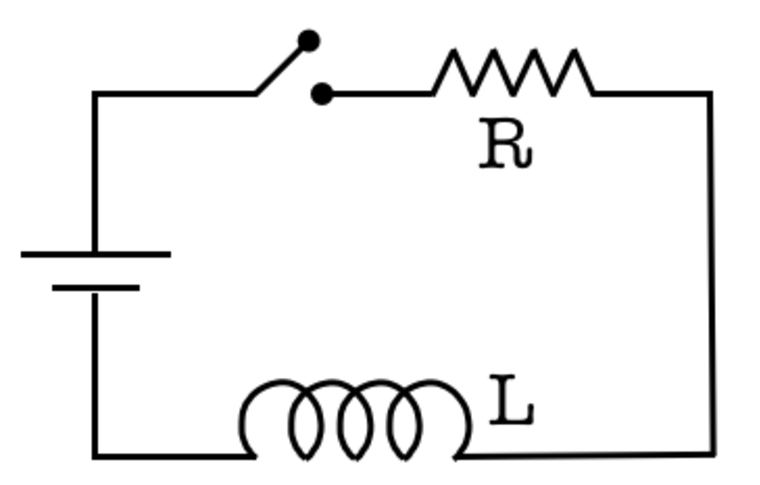
\includegraphics[width=0.4\textwidth]{RL}
%         \caption{\emph{Circuito R-L.}}\label{RL}
% \end{figure}
% Considerese el circuito que se muestra en la figura \ref{RL}, el cual se cierra en $t=0$. Al considerar el inductor se tiene
% \begin{equation}
% \xi+\xi_L&=&R\ I\nonumber\\
% \xi-L\dfrac{dI}{dt}&=&R\ I\, ,
% \end{equation}
% así que
% \begin{equation} \label{ecI}
% \dfrac{dI}{dt}+\dfrac{R}{L}I-\dfrac{\xi}{L}=0\, .
% \end{equation}
% Un truco para resolver esta última ecuación diferencial es derivar nuevamente, con lo cual se tiene
% \begin{equation}
% \dfrac{d^2I}{dt^2}+\mu\dfrac{dI}{dt}=0\, ,
% \end{equation}
% con $\mu=R/L$. La solución correspondiente es de la forma
% \begin{equation}
% I(t)=A+B \mbox{e}^{-\mu t}\, ,
% \end{equation}
% con $A$ y $B$ son constantes que se determinan enseguida. Si en $t=0$ se tiene $I(t=0)=0$, entonces se obtiene
% \begin{equation}
% B=-A,
% \end{equation}
% de esta forma
% \begin{equation}
% I(t)=A\left(1- \mbox{e}^{-\mu t} \right). \label{sI}
% \end{equation}
% Al sustituir (\ref{sI}) en (\ref{ecI}) se tiene
% \begin{equation}
% \mu\ A\ \mbox{e}^{-\mu t}+\mu A \left(1- \mbox{e}^{-\mu t} \right)-\dfrac{\xi}{L}=0\,,
% \end{equation}
% de lo cual se encuentra el valor de $A$
% \begin{equation}
% A=\dfrac{\xi}{R}.
% \end{equation}
% Finalmente se tiene la expresión de la corriente $I$
% \begin{equation}
% I(t)=\dfrac{\xi}{R}\left(1- \mbox{e}^{-\frac{R}{L} t} \right),
% \end{equation}
% la cantidad $\tau=L/R$ se conoce como {\it constante de tiempo}. El comportamiento de la corriente eléctrica se muestra en la figura \ref{I}.
% \begin{figure}[H]
% \centering
% \hspace{20pt}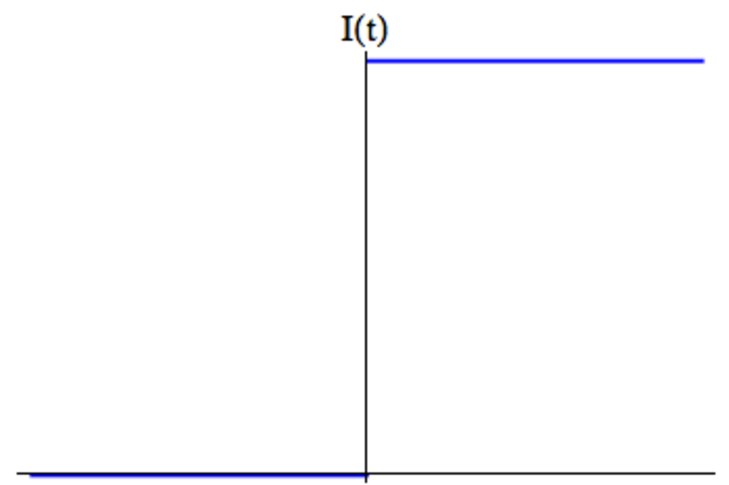
\includegraphics[scale=.4]{sinL}
% \hfill
% 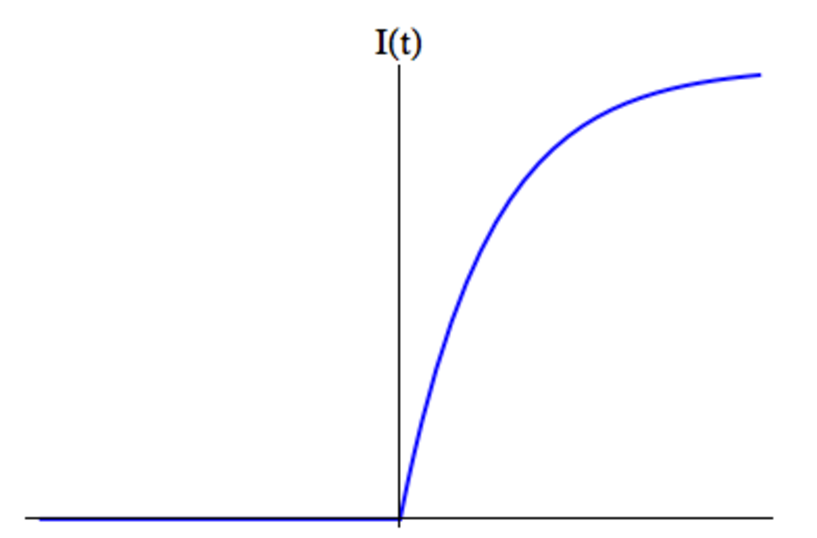
\includegraphics[scale=.35]{conL}
% \hspace{20pt}
% \caption{Comportamiento de $I(t)$ en presencia de una resistencia (izquierda) y con un inductor (derecha).} \label{I}
% \end{figure}
% \end{example}
%
%
% %%%%%%%%%%%%%%%%%%%%%%EJEMPLO%%%%%%%%%%%%%%%%%%%
% \begin{example}Circuito R-L-C.%\cite{RMC}
% El segundo ejemplo es considerar un circuito serie $R-L-C$ que se conecta repentinamente a un voltaje constante $V$. Este circuito se muestra en la figura \ref{RLC}
% \begin{figure}[ht]
%   \centering
%     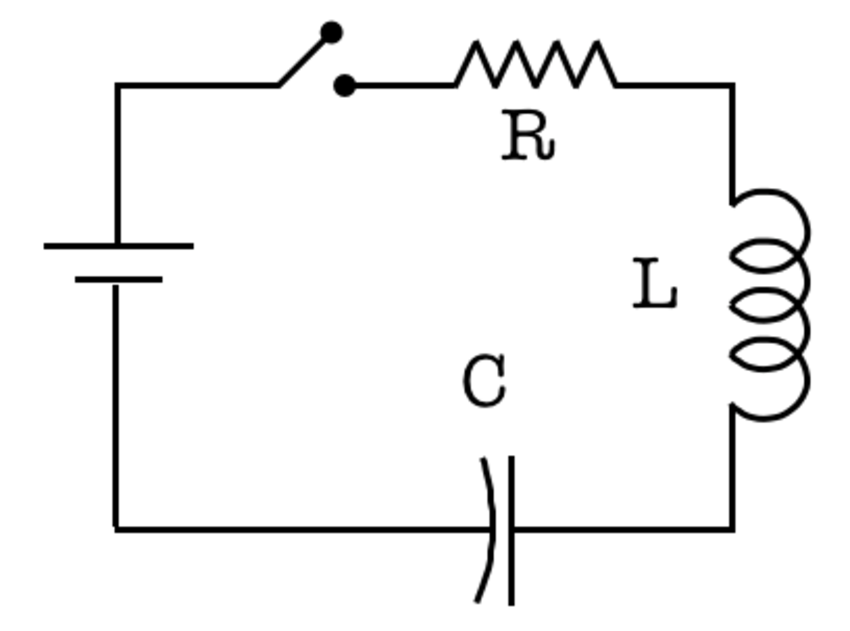
\includegraphics[width=0.35\textwidth]{RLC}
%         \caption{\emph{Circuito R-L-C.}}\label{RLC}
% \end{figure}
% Sabemos que el voltaje al que está sometida la resistencia es dado por $RI$, para el inductor es $-\frac{dI}{dt}$ y para el capacitor(consideramos la capacitancia constante) se determina observando que
% \begin{equation}
% I(t)=\dfrac{dQ}{dt}=\dfrac{d(CV)}{dt}=C\dfrac{dV}{dt},
% \end{equation}
% por lo cual
% \begin{equation}
% V=\dfrac{1}{C}\int^t_0 I(\tau)d\tau,
% \end{equation}
% así que
% \begin{equation}
% V=RI(t)+L\dfrac{dI(t)}{dt}+\dfrac{1}{C}\int^t_0 I(\tau)d\tau.\label{VT}
% \end{equation}
% Para resolver esta ecuación diferencial se hace un truco semejante al ejemplo anterior, esto es derivar nuevamente con respecto al tiempo:
% \begin{equation}
% \dfrac{dV}{dt}=R\dfrac{dI(t)}{dt}+L\dfrac{d^2I(t)}{dt^2}+\dfrac{1}{C} I(t),\label{dVdI}
% \end{equation}
% o bien, se puede escribir
% \begin{equation}
% \dfrac{dV}{dt}=\dfrac{d^2I(t)}{dt^2}+\dfrac{R}{L}\dfrac{dI(t)}{dt}+\dfrac{1}{CL} I(t).
% \end{equation}
% Para el caso en que $\frac{dV}{dt}=0$ se tiene la ecuación diferencial
% \begin{equation}
% \dfrac{d^2I(t)}{dt^2}+\dfrac{R}{L}\dfrac{dI(t)}{dt}+\dfrac{1}{CL} I(t)=0, \label{IRCL}
% \end{equation}
% las raíces del polinomio característico son
% \begin{equation}
% r_\pm=-\dfrac{R}{2L}\pm\sqrt{\dfrac{R^2}{4L^2}-\dfrac{1}{CL}}.
% \end{equation}
% Al definir
% \begin{equation}
% \omega_n=\sqrt{\dfrac{1}{CL}-\dfrac{R^2}{4L^2}},
% \end{equation}
% se tiene
% \begin{equation}
% r_\pm=-\dfrac{R}{2L}\pm i\ \omega_n.
% \end{equation}
% Con esto, las soluciones de (\ref{IRCL}) son de la forma
% \begin{equation}
% I(t)=\Big(A\ \mbox{e}^{i\ \omega_n\ t}+B\ \mbox{e}^{-i\ \omega_n\ t} \Big) \mbox{e}^{-\frac{R}{2L}t},
% \end{equation}
% con $A$ y $B$ constantes.
% Si $I(t=0)=0$ entonces $B=-A$, por lo cual
% \begin{equation}
% I(t)=D \sin(\omega_n\ t) \mbox{e}^{-\frac{R}{2L}t},\label{ID}
% \end{equation}
% con $D$ una constante que se determina usando (\ref{VT}) para el tiempo $t=0$:
% \begin{equation}
% V=L\dfrac{dI(t)}{dt}\Bigg|_{t=0},
% \end{equation}
% pero de (\ref{ID}) se tiene
% \begin{equation}
% \dfrac{dI(t)}{dt}\Bigg|_{t=0}=D\ \omega_n,
% \end{equation}
% entonces
% \begin{equation}
% D=\frac{V}{L \omega_n}.
% \end{equation}
% Finalmente se tiene la forma completa de la corriente
% \begin{equation}
% I(t)=\frac{V}{L \omega_n}\sin(\omega_n\ t)\ \mbox{e}^{-\frac{R}{2L}t},
% \end{equation}
% cuyo comportamiento se muestra en la figura \ref{IRLC}.
% \begin{figure}[H]
%   \centering
%     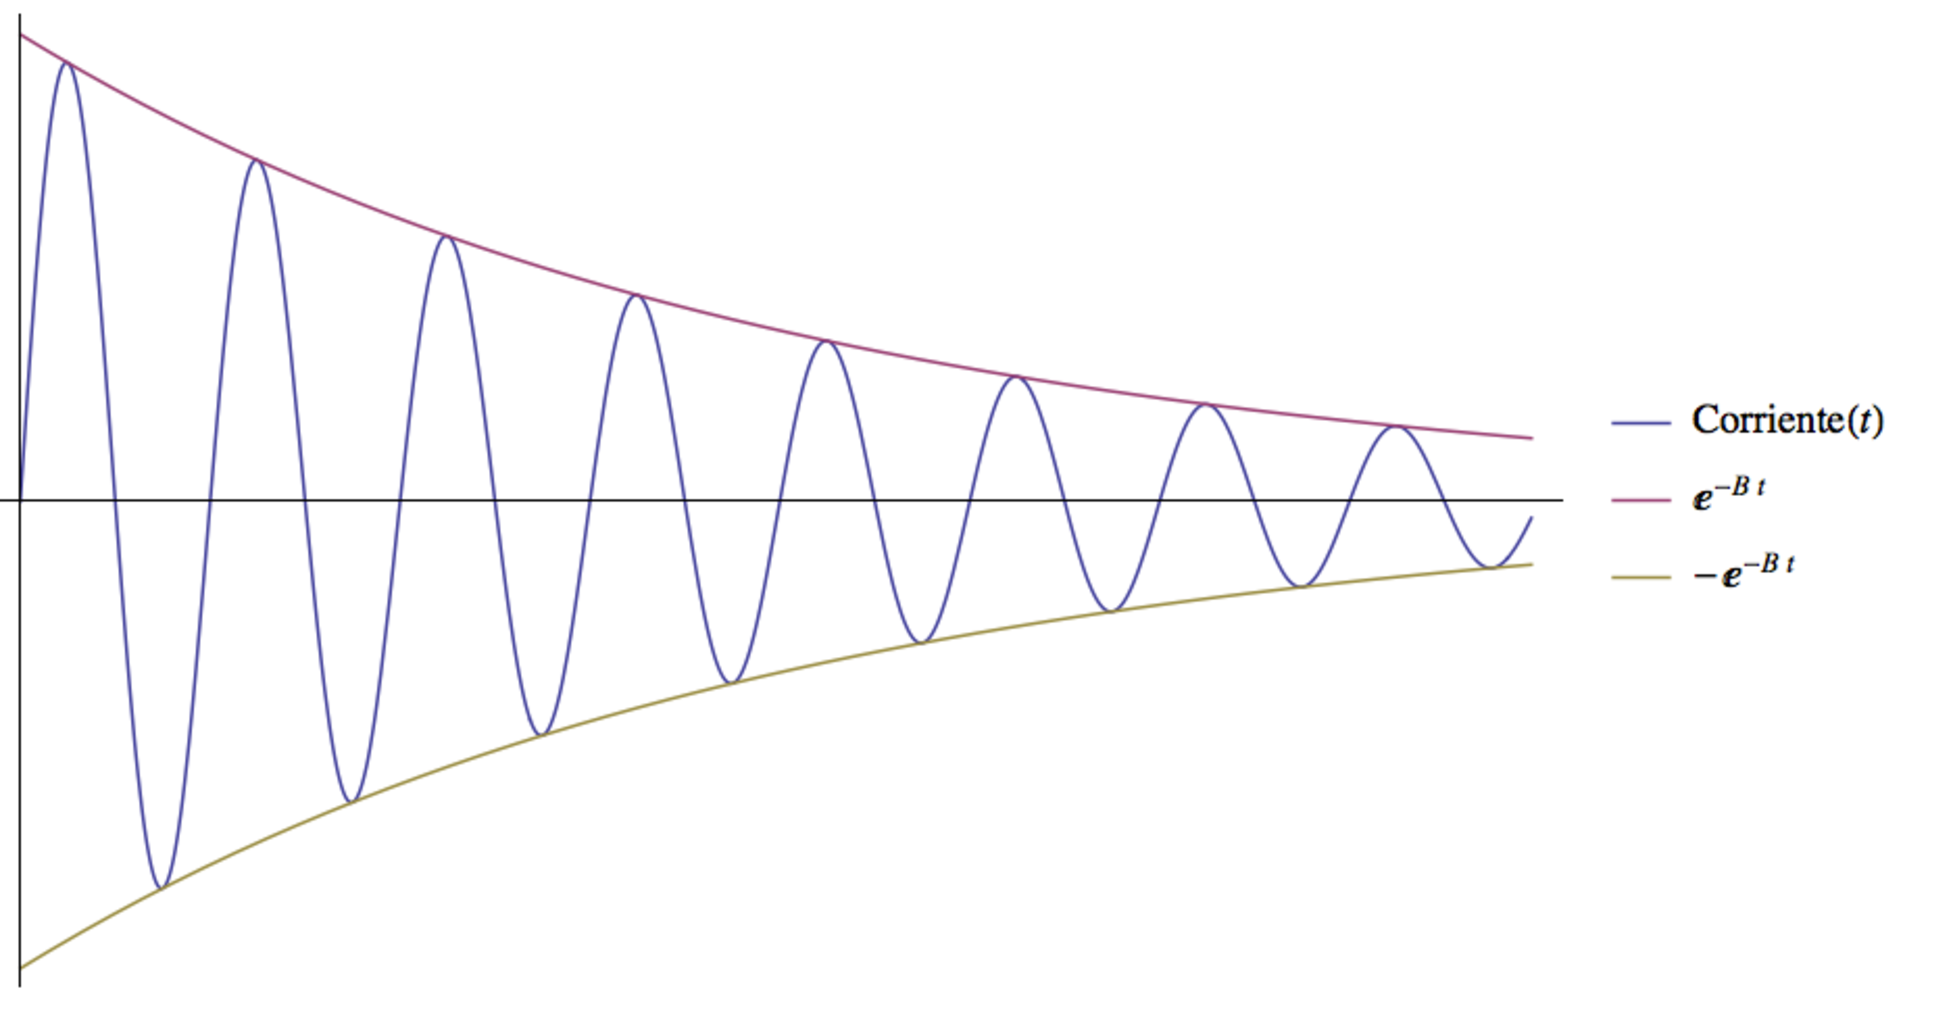
\includegraphics[width=0.7\textwidth]{IRLC}
%         \caption{\emph{Comportamiento de la corriente para el circuito R-L-C.}}\label{IRLC}
% \end{figure}
%
% Es sencillo observar que en el caso cuando $R=0$ se tiene una corriente dada por
% \begin{equation}
% I(t)=V \sqrt{\frac{C}{L}}\ \sin\left(\dfrac{1}{\sqrt{CL}}\ t\right),
% \end{equation}
% este caso tan sencillo es importante ya que está presente en la {\it bobina de Tesla}.
% \end{example}
%
%
%
% %%%%%%%%%%%%%%%%%%%%%%EJEMPLO%%%%%%%%%%%%%%%
% \begin{example}: En este ejemplo se usa nuevamente el circuito RLC pero con un voltaje dado por $V(t)=V_0\ \cos(\omega t)$. El truco que ahora se usa consiste en introducir {\it corrientes ficticias} a partir de la ec. (\ref{dVdI}):
% \begin{equation}
% \dfrac{dV_1}{dt}+i\dfrac{dV_2}{dt}=\left(L\dfrac{d^2I_1}{dt^2}+R\dfrac{dI_1}{dt}+\dfrac{I_1}{C}\right)+i\left(L\dfrac{d^2I_2}{dt^2}+R\dfrac{dI_2}{dt}+\dfrac{I_2}{C}\right).\label{Iim}
% \end{equation}
% Dada la forma de $V(t)$, el lado derecho de (\ref{Iim}) se simplifica considerablemente al usar $V(t)=V_0\ \mbox{e}^{i\omega t}$ y a partir de esta expresión se puede deteminar la corriente $I(t)$:
% \begin{equation}
% I(t)=C\dfrac{dV}{dt}=iC\ V_0\ \omega\ \mbox{e}^{i\omega t}=I_0 \mbox{e}^{i\omega t},\label{IComplex}
% \end{equation}
% con $I_0=iC\ V_0\ \omega$. Entonces la ec. (\ref{Iim}) se escribe de la forma
% \begin{equation}
% i\omega V_0\ \mbox{e}^{i\omega t}&=&\left[L \big(-\omega^2 I_0\ \mbox{e}^{i\omega t}\big)+R \big(i\omega I_0 \ \mbox{e}^{i\omega t}  \big) +\dfrac{I_0}{C} \ \mbox{e}^{i\omega t}  \right]\nonumber\\
% &=&\left[-\omega^2 L+i R +\dfrac{1}{C}\right]I_0 \ \mbox{e}^{i\omega t}.
% \end{equation}
% Al multiplicar esta última expresión por $-\frac{i}{\omega}$
% \begin{equation}
% V_0 =\left[R +i\left(\omega L-\dfrac{1}{\omega C}\right)\right]I_0.\label{VoIo}
% \end{equation}
% Se define la {\bf impadencia}, Z, del circuito como la cantidad compleja
% \begin{equation}
% Z:=R +i\left(\omega L-\dfrac{1}{\omega C}\right),
% \end{equation}
% la parte real es la {\bf resistencia} ($R$) y la parte compleja es la {\bf reactancia} ($X$). La reactancia a su vez se divide en  {\bf reactancia inductiva}
% \begin{equation}
% X_L:=\omega L,\label{XL}
% \end{equation}
%  y la {\bf reactancia capacitiva}
% \begin{equation}
% X_C:=-\dfrac{1}{\omega C}.\label{XC}
% \end{equation}
% El comportamiento de $X_L$ y $X_C$ se muestra en la figura \ref{xlxc}.
% \begin{figure}[ht]
%   \centering
%     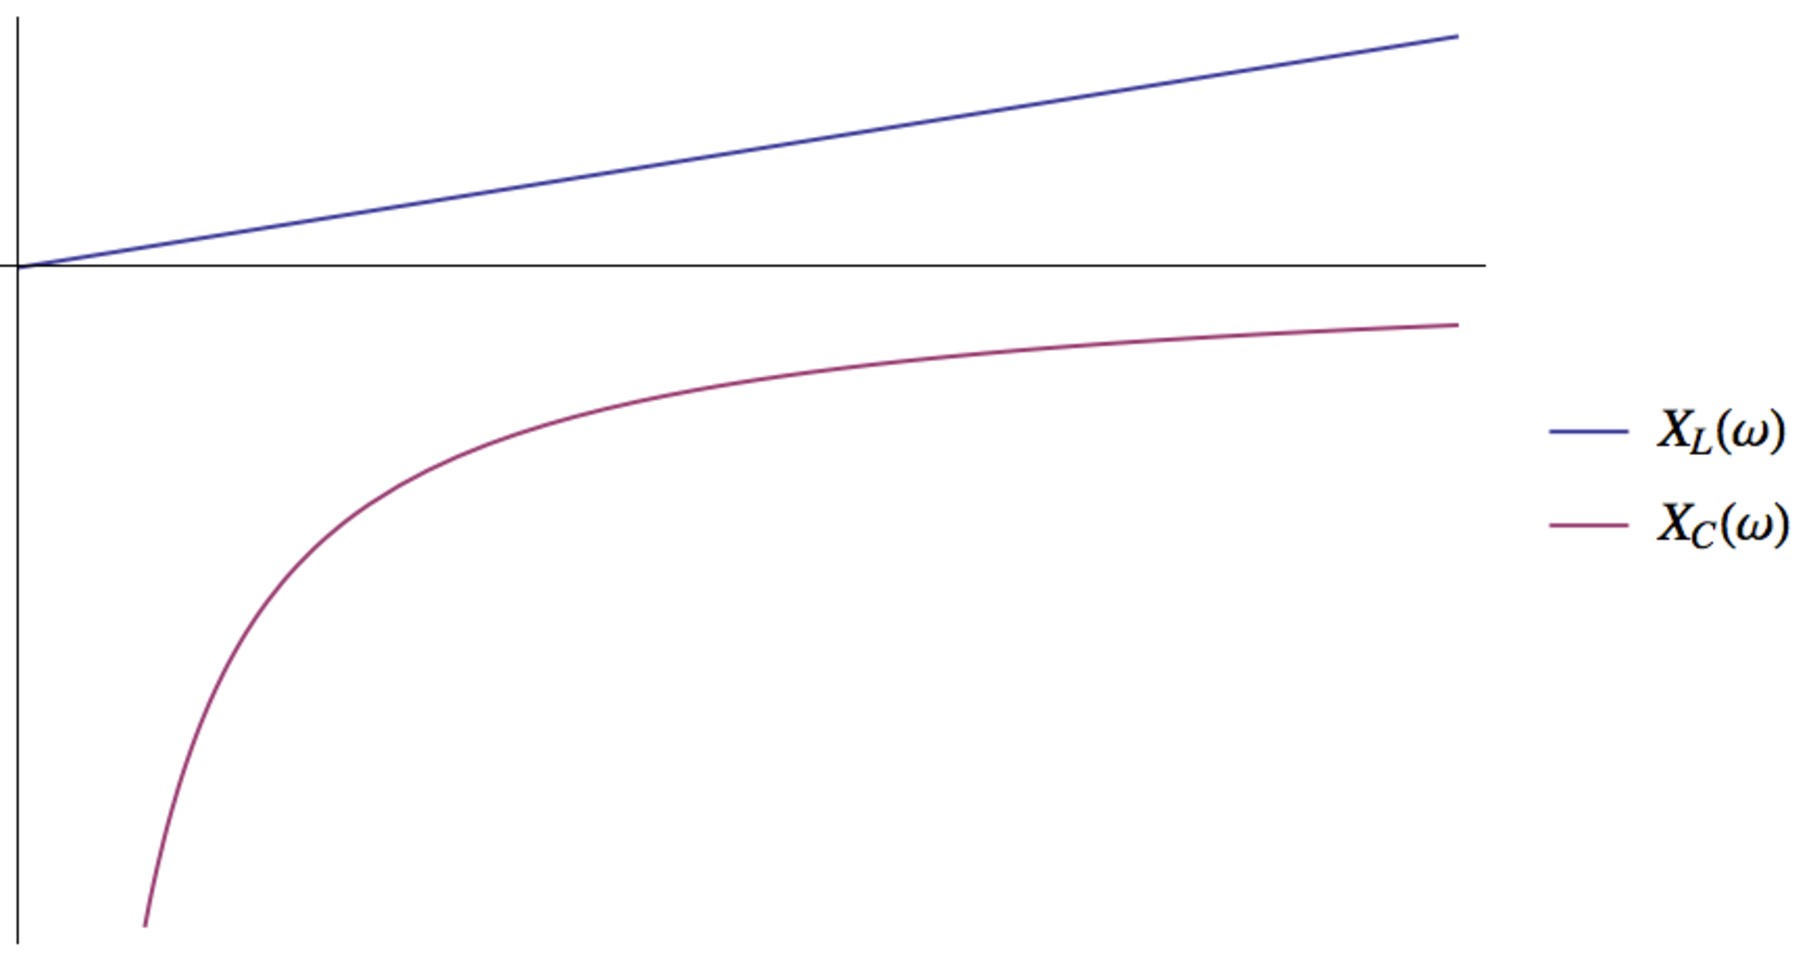
\includegraphics[width=0.6\textwidth]{XLXC}
%         \caption{\emph{Comportamiento de las reactancias.}}\label{xlxc}
% \end{figure}
%
% Al escribir la impadencia en su forma polar
% \begin{equation}
% Z=|Z|\mbox{e}^{i\theta},
% \end{equation}
% con
% \begin{equation}
% |Z|^2=R^2 +\left(\omega L-\dfrac{1}{\omega C}\right)^2,
% \end{equation}
% y
% \begin{equation}
% \theta=\tan^{-1}\left(\dfrac{\omega L-\dfrac{1}{\omega C}}{R}\right).
% \end{equation}
% Al usar la forma polar de la impedancia en la ec. (\ref{VoIo}) y sustituir $I_0$ en la ec. (\ref{IComplex}) se tiene
% \begin{equation}
% I(t)=\dfrac{V_0}{|Z|}\cos(\omega\ t-\theta).
% \end{equation}
% Si $\theta$ es mayor que cero, la corriente alcanza una fase dada más tarde que el voltaje y se dice que se retrasa con respecto al voltaje. En caso contrario, la corriente se adelanta al voltaje.
% \end{example}
%
%
%
%
%
%
% %%%%%%%%%%%%%%%%%SECTION%%%%%%%%%%%%%%%%%%%%%%
% \section{Transformador} \label{Transformador}
% Este dispositivo se hace con dos (o mas) embobinados distintos sobre un solo núcleo, por lo general de fierro o ferrita.
% \begin{figure}[ht]
%   \centering
%     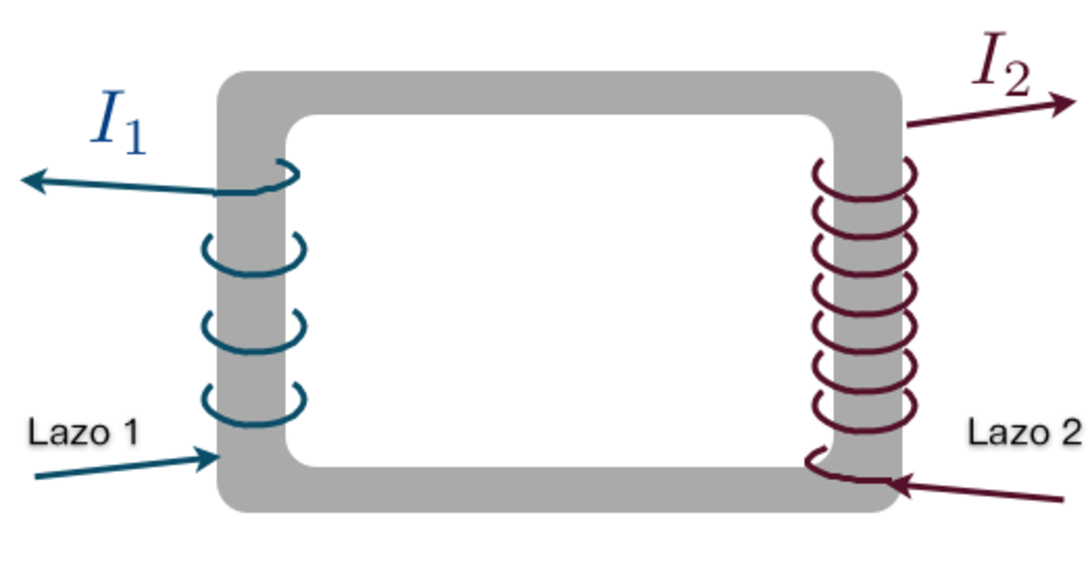
\includegraphics[width=0.5\textwidth]{transf}
%         \caption{\emph{Transformador.}}
% \end{figure}
%
% \subsection{Transformador perfecto}
% Esta sección es extraída de \cite{MA}. No presenta pérdidas de energía y el flujo producido por un embobando es interceptado por el otro. Llamaremos a los embobinados primario, $N_1$ vueltas, y el secundario, $N_2$ vueltas.
%
% Al considerar que todo el flujo de un embobando es interceptado por el otro, estamos diciendo que el flujo a través de cada vuelta de cada embobando es exactamente el mismo ($\Phi_1=\Phi_2=\Phi$)
% \begin{equation}
% V_1=\xi_1=-N_1 \dfrac{d\Phi}{dt}\ \ \ &\text{y}& \ \ \ V_2=\xi_2=-N_2 \dfrac{d\Phi}{dt},\\
% \dfrac{V_1}{V_2}&=&\dfrac{N_1}{N_2},
% \end{equation}
% o bien
% \begin{equation}
% V_2=\dfrac{N_2}{N_1} V_1. \label{v2v1}
% \end{equation}
% Para aumentar el voltaje, hay que mentar el número de vueltas (aumentamos el flujo y el cambio de flujo).
%
% El transformador es un elemento pasivo, y no puede proporcional más potencia en el secundario que la provista en el primario (por conservación de la energía). En el transformador ideal, la potencial del secundario es igual al a potencia en el primario:
% \begin{equation}
% P_1=V_1\ I_1, \ \ \ P_2=V_2\ I_2,
% \end{equation}
% entonces
% \begin{equation}
% V_1\ I_1=V_2\ I_2, \label{i2i1}
% \end{equation}
% al usar (\ref{v2v1}) en (\ref{i2i1}) se encuentra
% \begin{equation}
% I_1\ N_1=I_2\ N_2.
% \end{equation}
%
%
% %%%%%%%%%%%%%%%%%%%EJEMPLO%%%%%%%%%%%%%%%%%%
% \begin{example}: La energía eléctrica para consumo doméstico o industrial se transporta en forma de corriente alterna, debido principalmente a que es fácil generar corriente alterna con un generador mediante la {\it ley de Faraday}, pero sobre todo que puede producirse las pérdidas por {\it efecto Joule} al trasmitirla de esta manera. Pongamos por ejemplo, que una planta generadora de electricidad quiere trasmitir $100 \ KW$ a una distancia de $10\ Km$, mediante un cable de cobre de $26\ mm$ de diámetro.\\
% {\it Sol.} La potencia recibida en el destino ($P_f$) será la potencia a la que se manda la energía ($P_i$) menos las pérdidas por efecto Joule en el cable:
% \begin{equation}
% P_f=P_i-I^2\ R.
% \end{equation}
% La resistencia del cable se obtiene de
% \begin{equation}
% R=\dfrac{l}{A} \eta,
% \end{equation}
% donde $l$ es la longitud del cable, $A$ es el área seccional y $\eta$ es la resistividad. Entonces
% \begin{equation}
% A&=&5.309\times 10^{-4}\ m^2,\\
% \eta&=&1.7\times 10^{-8}\ \Omega\ m,
% \end{equation}
% así
% \begin{equation}
% R=l(3.202 \times 10^{-5}\Omega/m).
% \end{equation}
%
% Si la trasmisión se hace en corriente directa, a $100\ V$, la corriente sería
% \[I=\dfrac{P}{V}=1000 A,\]
% y las pérdidas por efecto Joules serían
% \begin{equation}
% I^2\ R = l(32.02\ W/m).
% \end{equation}
%
% Dado que $P=I^2\ R$ y $P=100\ KW$, entonces
% \[l=\dfrac{100 000\ W}{32.02\ W/m }=3.123\ Km\ !\]
%
%
% Supongamos que la planta tiene un transformador que eleva el voltaje a $100 000\ V$ para trasmitirla a $1\ A$ de corriente. Las pérdidas en este caso:
% \begin{equation*}
% I^2\ R &=& (1\ A^2)\ l \ (3.202 \times 10^{-5} \Omega/m)\\
% &=&l(3.202\times10^{-5}W/m),
% \end{equation*}
% por lo cual
% \[l=\dfrac{100 000\ W}{3.202\times10^{-5}W/m}=3.123 \times10^6\ Km.\]
% Al trasmitir $100\ KW$ una distancia de $10 Km$ las párdidas son
% \[I^2\ R= (10 000\ m) (3.202\times10^{-5}W/m)=0.3202\ W.\ !\]
% Al llegar al destino, se tiene un transformador que baja el voltaje. Si el voltaje baja a $100\ V$, entonces se tiene $1000\ A$.
% \end{example}
%
%
% %%%%%%%%%%%%%%%%%%SECCION%%%%%%%%%%%%%%%%%%
% \subsection{Transformador real}
% Esta sección es extraída de \cite{MA}. En un transformador real no toda la potencia del primer bobinado se transfiere al secundario, esto es debido a la existencia de corrientes parásitas\footnote{Ver apéndice \ref{ParasitasI}}.  Otras pérdidas de energía se representan por la resistencia finita de los alambres de los embobinados y además por la capacitancia parásita\footnote{Ver apéndice \ref{ParasitasC}} entre cada una de la vueltas.
%
% La representación de un transformador real se muestra en la figura \ref{TR}.
% \begin{figure}[ht]
%   \centering
%     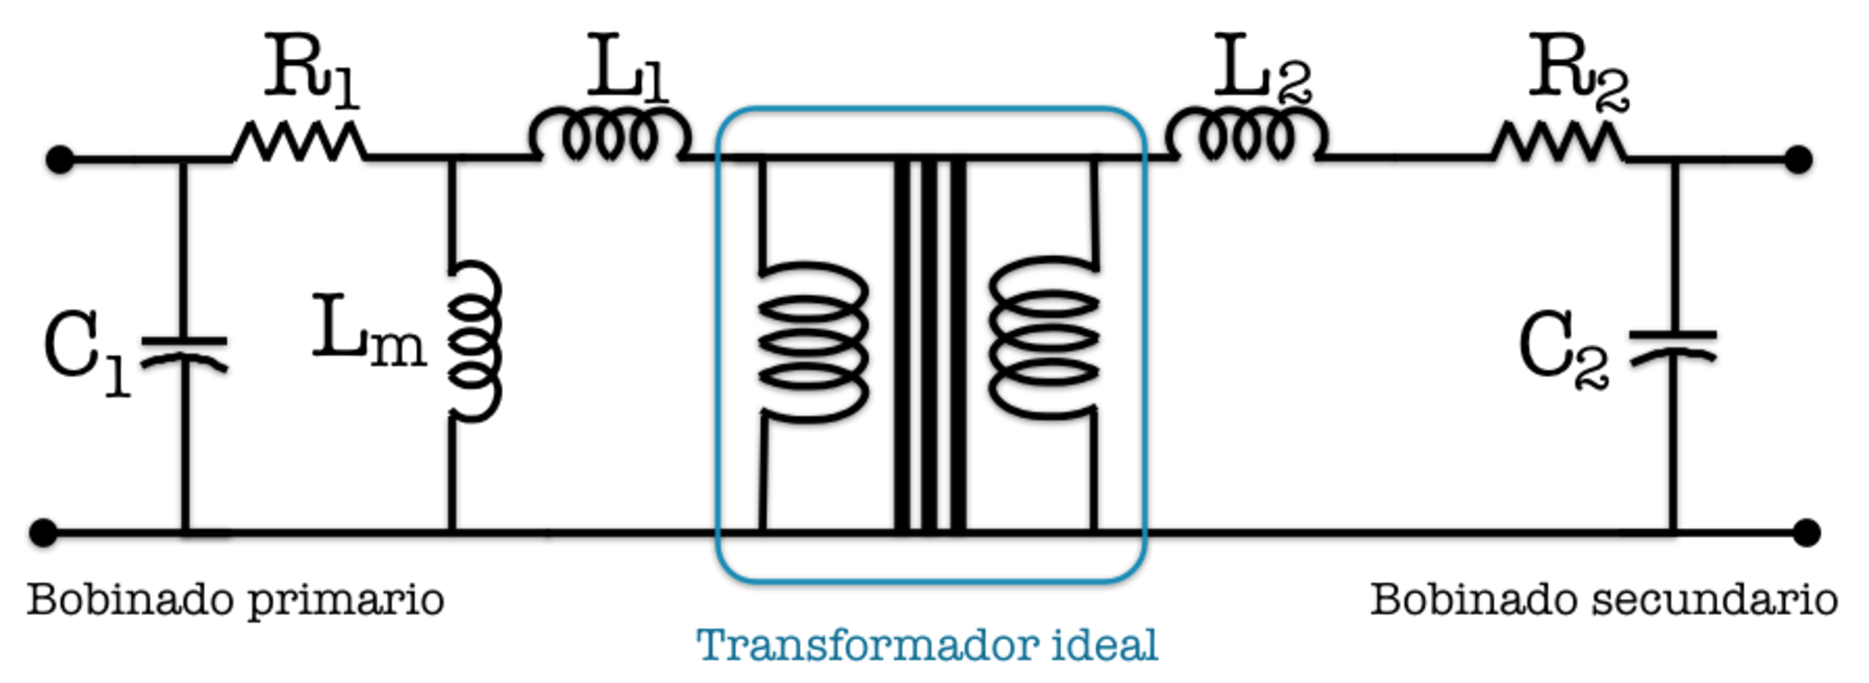
\includegraphics[width=0.7\textwidth]{TransR}
%         \caption{\emph{Transformador real.}}\label{TR}
% \end{figure}
% Las inductancias $L_1$ y $L_2$ representan la parte del flujo no interceptado por el otro embobinado, $R_1$ y $R_2$ son las resistencias de los embobinados, y $C_1$ y $C_2$ indican las capacitancias de los mismos.  La inductancia $L_m$ es la asociada con el flujo de corriente en {\color{red} situación de circuito abierto en el secundario}.
%
% A bajas frecuencias, la mayor parte de la energía se pierde en la magnetización del núcleo y por la capacitancia párasita, mientras que a altas frecuencias la mayoría se pierde por los inductancias $L_1$ y $L_2$ (ver la ec. (\ref{XL}) para este último argumento). Así que los transformadores reales son dise\~nados para operar en cierto rango de frecuencias. También se pierde energía en el núcleo ya que toda la enería usada en la magnetización no se recupera.
%
% La potencia entregada al bobinado secundario por el primario, se expresa mediante
% \begin{equation}
% P_2=e\,P_1,
% \end{equation}
% donde $e$ es el {\it factor de eficiencia}.
%
%
% %*********************SECCION********************
% \section{Energía almacenada en un sistema de solenoides con corrientes estacionarias}
% Consideremos un sistema de corrientes libres de un grupo de $n$ circuitos rígidos y fijos en el espacio. Se desea calcular el trabajo necesario para comenzar de una situacio\'n en la que todas las corrientes son cero y terminar en una situación en la que la corriente del circuito $Ci$ tenga un valor final $I_i$, siendo $i=1,2,...,n$.\\
% \\
% Supóngase que al tiempo $0<t<t_f$ la corriente de cada circuito $C_i$ está dada por
% \begin{equation}
% i_i&=&\frac{dq_i}{dt},
% \end{equation}
% de modo que no han alcanzado su valor final $I_i$. Un cambio en una de las corrientes en un lapso de tiempo $dt$ provocará un cambio en el flujo $d\Phi_i$ a través de  $C_i$ y de acuerdo con (\ref{ley de faraday}) provocará también una fem inducida. A fin de mantener el sistema, una fuente externa debe suministrar una fem igual a este valor pero en sentido opuesto, de esta forma, el trabajo realizado por la fuente externa será
% \begin{equation}
% dW_{ext,\,\,i}&=&\xi_{ext}\,\,dq_i,\nonumber\\
% &=&-\xi_{i,\,ind}\,\,i_i\,dt.
% \end{equation}
% Usando (\ref{ley de faraday}) se tiene que el trabajo realizado por la fuente externa es
% \begin{equation}
% dW_{ext,\,\,i}&=&i_i\,\,d\Phi_i.
% \end{equation}
% Al sumar la contribución de todas las corrientes se encuentra que el trabajo total, y por lo tanto, la energía magnética será
% \begin{equation}
% dW_{ext}&=&dU_{m}\,\,\,=\,\,\,\sum_{i=1}^n i_i\,\,d\Phi_i.\label{Wtot iq Um}
% \end{equation}
% Dado que los circuitos son constantes en forma y configuración, la única manera en la que los flujos pueden cambiar es que haya cambios en la corrientes, entonces de (\ref{fluj tot en Ci inclu C_i})
% \begin{equation}
% d\Phi_i&=&\sum_{j=1}^nM_{ij}\,di_j.
% \end{equation}
% Al combinar con (\ref{Wtot iq Um}) se obtiene
% \begin{equation}
% dU_{m}&=&\sum_{i=1}^n \sum_{j=1}^n M_{ij}\,i_i\,di_j.\label{dUm}
% \end{equation}
% Ahora supóngase que al instante dado $t$, cada una de las corrientes se encuentra a la misma fracción $f$ de su valor final, de tal forma que
% \begin{equation}
% i_i(t)&=&f(t)\, I_i.
% \end{equation}
% Entonces
% \begin{equation}
% di_j&=&I_j\,df,
% \end{equation}
% así, de (\ref{dUm}) se tiene que
% \begin{equation}
% dU_{m}&=&\sum_{i=1}^n \sum_{j=1}^n M_{ij}\,I_iI_j\,f\,df,\nonumber\\
% \Rightarrow U_{m}&=&\sum_{i=1}^n \sum_{j=1}^n M_{ij}\,I_iI_j\int_0^1f\,df,\nonumber\\
% &=&\frac{1}{2}\sum_{i=1}^n \sum_{j=1}^n M_{ij}\,I_iI_j.
% \end{equation}
% Utilizando nuevamente (\ref{fluj tot en Ci inclu C_i})
% \begin{equation}
% U_{m}&=&\frac{1}{2}\sum_{i=1}^n \,I_i\Phi_i.\label{energia magnetica}
% \end{equation}
% Siendo $\Phi_i$ el flujo total a través de $C_i$ proveniente de todas las fuentes, incluyendo ella misma.\\
% \\
% Podemos expresar la energía magnética en término de distribuciones de corriente. Recordamos de (\ref{flujo en term d A teor Sto}) que
% \begin{equation}
% \Phi&=&\oint_C\textbf{A}(\textbf{r})\cdot \dl \textbf{l}.\nonumber
% \end{equation}
% Sustituyendo en (\ref{energia magnetica}) se obtiene
% \begin{equation}
% U_{m}&=&\frac{1}{2}\sum_{i=1}^n \oint_{C_i}\textbf{A}(\textbf{r}_i)\cdot I_i\,\dl \textbf{l}_i,\label{energia magnetica en term A}
% \end{equation}
% donde $\textbf{A}(\textbf{r}_i)$ es el potencial vectorial total en $\textbf{r}_i$ del elemento de corriente $I_i\,\dl \textbf{l}_i$ de $C_i$. La suma sobre $i$ es la contribución de todos los elementos de corriente de todo el sistema. Por otro lado, recordamos también la equivalencia (\ref{elementos de corriente eq})
% \begin{equation}
% I\,\dl \textbf{l}&=&\textbf{J}\,dv\,\,\,=\,\,\,\textbf{K}\,da.\nonumber
% \end{equation}
% Se debe tener en cuenta que se están manejando corrientes libres, en consecuencia se debe integrar con respecto a todas las regiones que contienen corrientes, así de (\ref{energia magnetica en term A})
% \begin{equation}
% U_{m}&=&\frac{1}{2}\int_{S}\textbf{K}_l(\textbf{r})\cdot\textbf{A}(\textbf{r})\,da.\label{energia magnetica dist sup}
% \end{equation}
% En las regiones en las que no hay corriente $\textbf{K}_l=0$, de esta forma se puede extender la región de integración para cubrir todo el espacio, con lo que la energía magnética se puede expresar como
% \begin{equation}
% U_{m}&=&\frac{1}{2}\int_{todo\,el\,espacio}\textbf{K}_l(\textbf{r})\cdot\textbf{A}(\textbf{r})\,da.\label{energia magnetica sup}
% \end{equation}
% Si existen corrientes volumétricas
% \begin{equation}
% U_{m}&=&\frac{1}{2}\int_{todo\,el\,espacio}\textbf{J}_l(\textbf{r})\cdot\textbf{A}(\textbf{r})\,d\mbox{v}.\label{energia magnetica volumetrica}
% \end{equation}
%
%
% %*********************SECCION********************
% \section{Densidad de energía y tensor de esfuerzos de Maxwell en el campo magnetostático}
% Como se están considerando corrientes libres podemos ocupar (\ref{forma diferencial ley de ampere})
% \begin{equation}
% \nabla\times\B&=&\mu_0\,\textbf{J},\nonumber
% \end{equation}
% para expresar (\ref{energia magnetica volumetrica}) como
% \begin{equation}
% U_{m}&=&\frac{1}{2\mu_0}\int_{todo\,el\,espacio}(\nabla\times\B)\cdot\textbf{A}\,d\mbox{v},\label{um rot b}
% \end{equation}
% donde
% \begin{equation}
% (\nabla\times\B)\cdot\textbf{A}&=&\B\cdot(\nabla\times \textbf{A})-\nabla\cdot(\textbf{A}\times\B).
% \end{equation}
% Sustituyendo en (\ref{um rot b}) y usando $\B=\nabla\times\textbf{A}$ se tiene
% \begin{equation}
% U_{m}&=&\frac{1}{2\mu_0}\int_{V}\B^2\,d\mbox{v}-\frac{1}{2\mu_0}\int_{V}\nabla\cdot(\textbf{A}\times\B)\,d\mbox{v}.
% \end{equation}
% Usando el teorema de la divergencia en la segunda integral se obtiene
% \begin{equation}
% U_{m}&=&\frac{1}{2\mu_0}\int_{V}\B^2\,d\mbox{v}-\frac{1}{2\mu_0}\oint_{S}(\textbf{A}\times\B)\cdot da.\label{um con v y s}
% \end{equation}
% Se debe considerar a $V$ como un volumen muy grande y $S$ como su superficie de frontera. A medida que $V\rightarrow\infty$, $S$ también se extiende hasta el infinito. Podemos observar de (\ref{potencial magnetico volumetrico}) y (\ref{induccion mag de una dist volumetrica}) que
% \begin{equation}
% \textbf{A}\sim\frac{1}{R}\,\,\,\,,\,\,\,\,\B\sim\frac{1}{R^2}
% \end{equation}
% A medida que $R\rightarrow\infty$ observamos que la segunda integral de (\ref{um con v y s}) se anula
% \begin{equation}
% \oint_{S}(\textbf{A}\times\B)\cdot da\sim\frac{1}{R^3}\cdot R\sim\frac{1}{R}\longrightarrow 0,
% \end{equation}
% con lo que la energía magnética queda como
% \begin{equation}
% U_{m}&=&\frac{1}{2\mu_0}\int_{todo\,el\,espacio}\B^2\,d\mbox{v}.\label{magnetic energy}
% \end{equation}
% La energía magética se encuentra distribuida en forma continua a través del espacio con una \emph{densidad de energía} dada por
% \begin{equation}
% u_{m}&=&\frac{1}{2\mu_0}\B^2,\label{densidad energia mag}
% \end{equation}
% de manera que
% \begin{equation}
% U_{m}&=&\int_{todo\,el\,espacio}u_m\,d\mbox{v}.\label{densidad magnetic energy}
% \end{equation}
% Las unidades de $u_m$ son $joule/metro^3$.\\
% \\
% Supongamos ahora que una parte del sistema efectúe un desplazamiento $\dl \textbf{r}$ bajo la influencia de las fuerzas magnéticas sobre él, permaneciendo constantes todas las corrientes. El trabajo mecánico efectuado por la fuerza $\textbf{F}$ que actúa sobre el sistema es
% \begin{equation}
% dW&=&\textbf{F}\cdot \dl \textbf{r}.\label{trab mec caso magnetico}
% \end{equation}
%  Cuando los circuitos se mueven con respecto a otro, se registrará un cambio en los flujos a través de ellos, lo que provocará la existencia de una fem inducida y, para que las corrientes se mantengan constantes, las fuentes externas deberán realizar trabajo en contra de la fem. En estas circunstancias, al igual que en el caso eléctrico el trabajo tiene dos contribuciones como en la ec. (\ref{W electrico con Wex y Uelec}), así el trabajo realizado por el sistema y las fuentes externas de energía resulta ser
% \begin{equation}
% dW&=&dW_{ext}-dU_m,\label{Wtot mag Wext Um}
% \end{equation}
% donde $dU_m$ es el cambio en la energía magnética del sistema y $dW_{ext}$ es el trabajo realizado por las fuentes de energía externas para mantener las corrientes constantes.\\
%
% Ya se encontró en (\ref{Wtot iq Um}) el trabajo que deben proporcionar las fuentes externas, sin embargo, se debe recordar que en este caso las corrientes ya se encuentran en sus estados finales, de esta forma
% \begin{equation}
% dW_{ext}&=&\sum_{i=1}^n I_i\,\,d\Phi_i\nonumber\\
% &=&2\,dU_m.
% \end{equation}
% Donde se usó (\ref{energia magnetica}). Sustituyendo en (\ref{Wtot mag Wext Um}) y combinando con (\ref{trab mec caso magnetico}) obtenemos
% \begin{equation}
% dU_m&=&\textbf{F}\cdot \dl \textbf{r}.\\
% \Rightarrow \textbf{F}&=&(\nabla U_m)_{I}.\,\,\,\,\,\,\,\,\,\,\,\,\,\,\,\,\,\,\,\,\,(corrientes\,\,\,constantes)\label{fza iq grad de Um corr cte}
% \end{equation}
% Si el circuito se restringe a moverse de tal modo que gire en torno a un eje, la ec. (\ref{trab mec caso magnetico}) puede sustituirse por
% \begin{equation}
% dW&=&\pmb{\tau}\cdot d\pmb{\theta},
% \end{equation}
% donde $\pmb{\tau}$ es el momento magnético sobre el circuito y $d\pmb{\theta}$ es un desplazamiento angular. En estas condiciones
% \begin{equation}
% \tau_i&=&\left(\frac{\partial U_m}{\partial\theta_i} \right)_I.\label{torq iq grad de Um corr cte}
% \end{equation}
% En algunos otros casos, los flujos que atraviesan los circuitos pueden mantenerse constantes en lugar de las corrientes, con lo cual no se requerirá de un cambio en las fuentes de energía externas, de manera que $dW_{ext}=0$ en (\ref{Wtot mag Wext Um}), así
% \begin{equation}
% dW&=&-dU_m,\\
% \Rightarrow dU_m&=&-\textbf{F}\cdot \dl \textbf{r}.
% \end{equation}
% Por lo tanto
% \begin{equation}
%  \textbf{F}&=&-(\nabla U_m)_{\Phi}.\,\,\,\,\,\,\,\,\,\,\,\,\,\,\,\,\,\,\,\,\,(flujos\,\,\,constantes)\label{fza iq -grad de Um flujo cte}
% \end{equation}
% Y
% \begin{equation}
% \tau_i&=&-\left(\frac{\partial U_m}{\partial\theta_i} \right)_\Phi.\label{torq iq -grad de Um flujo cte}
% \end{equation}
%
%
%
%
% %*********************EJEMPLO********************
% \begin{example}
% Se da un circuito de corriente en un campo magnético prescrito. La fuerza magnética sobre cada elemento de circuito $\dl \textbf{l}$ está dada por $I\,\,d\textbf{l}\times\B$. Si el circuito se puede mover bajo las influencias de las fuerzas magnéticas, de tal modo que un elemento típico se desplaza $\delta r$ y al mismo tiempo la intensidad de la corriente $I$ se mantiene constante, demuestre por cálculo directo que el trabajo mecánico efectuado por el circuito es $\delta W=I\,\,\delta\Phi$, donde $\delta\Phi$ es el flujo adicional que atraviesa el circuito.\\
% \emph{Solución}.\\
% El trabajo mecánico se puede calcular como
% \begin{equation}
% \delta W&=&\textbf{F}\cdot\delta\textbf{r}.
% \end{equation}
% Por otro lado, la fuerza sobre un elemento de corriente es
% \begin{equation}
% \textbf{F}&=&I\,\,\dl \textbf{l}\times\B,
% \end{equation}
% Así, el trabajo mecánico
% \begin{equation}
% \delta W&=&I\,(\dl \textbf{l}\times\B)\cdot\delta\textbf{r},\nonumber\\
% &=&-I\,(\B\times \dl \textbf{l})\cdot\delta\textbf{r}.
% \end{equation}
% Usando la identidad vectorial
% \begin{equation}
% (\textbf{A}\times\B)\cdot\textbf{C}&=&\textbf{A}\cdot(\B\times\textbf{C}).
% \end{equation}
% Con lo que
% \begin{equation}
% \delta W&=&-I\,\B\cdot(\dl \textbf{l}\times\delta\textbf{r}),\nonumber\\
% &=&I\,\B\cdot(\delta\textbf{r}\times \dl \textbf{l}).
% \end{equation}
% De la definición de producto vectorial se tiene que la magnitud del producto cruz es igual al área del paralelogramo que tiene a $\dl \textbf{l}$ y $\delta\textbf{r}$ como lados, es decir,
% \begin{equation}
% |\delta\textbf{r}\times \dl \textbf{l}|&=&|\delta\textbf{r}|\,\,|d\textbf{l}|\,\sin\theta\,\,\,=\,\,\,\delta a.\\
% \Rightarrow \delta\textbf{r}\times \dl \textbf{l}&=&\delta\textbf{a}.
% \end{equation}
% De esta forma
% \begin{equation}
% \delta W&=&I\,\B\cdot \delta\textbf{a}.
% \end{equation}
% Usando la definición de flujo magnético, ec. (\ref{flujo madnetico}) se obtiene finalmente
% \begin{equation}
% \therefore\delta W&=&I\,\delta\Phi.
% \end{equation}
% \end{example}
%
%
%
% %*********************EJEMPLO********************
% \begin{example}
% Un circuito en forma de una vuelta de alambre de radio $b$ se coloca en el centro de una vuelta más grande de radio $a$, $b\ll a$. El circuito peque\~no se fija de modo que puede girar libremente en torno a uno de sus diámetros, localizándose este diámetro en el plano del circuito mayor. Los circuitos conducen corrientes estacionarias $I_b$ e $I_a$, respectivamente. Si el ángulo entre las normales de los dos circuitos es $\theta$ (figura \ref{circuito-giratorio}), calcule el momento de rotación sobre el circuito móvil.
% \begin{figure}[H]
%   \centering
%     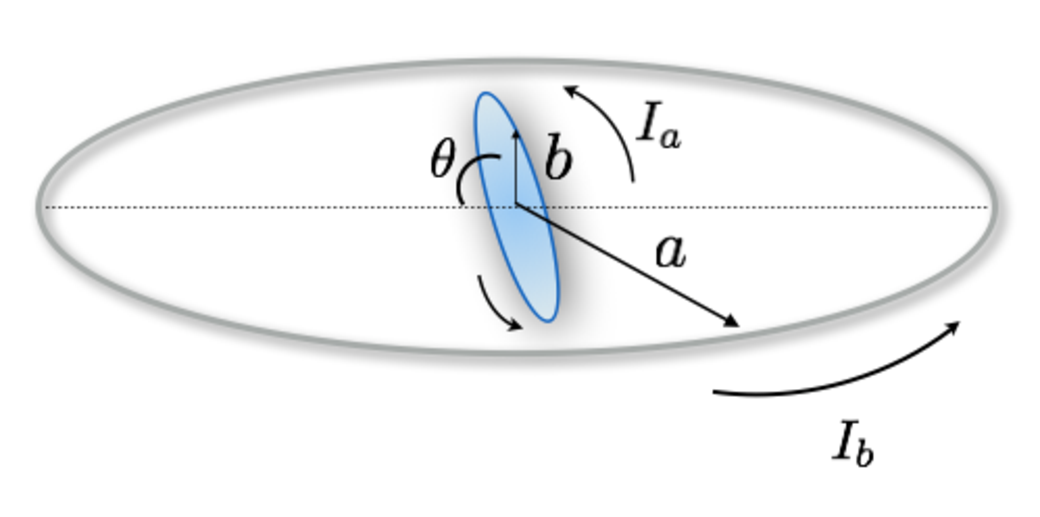
\includegraphics[width=0.45\textwidth]{circuito-giratorio}
%         \caption{\emph{Circuito de radio $b$ que gira en el centro de un circuito de radio $a$}}\label{circuito-giratorio}
% \end{figure}\\
% \emph{Solución.}\\
% Como el circuito de radio $b$ se mueve con respecto al otro, se registra un cambio en el flujo a través del mismo, lo cual provoca una fem inducida, pero en éste caso, las corrientes en los circuitos son estacionarias, de esta forma, debe existir una fuente externa que genere trabajo en contra de la fem para mantener a la corriente $I_a$ constante, este trabajo se puede obtener con la ec. (\ref{Wtot iq Um}), recordando que la corriente $I_a$ ya se encuentra en su estado fina, así
% \begin{equation}
% dU_{m}&=&I_b\,d\Phi,
% \end{equation}
% donde $d\Phi$ es el flujo que pasa a través del circuito de radio $b$, el cual es producido por el circuito de radio $a$. Podemos obtener este flujo, apartir de la ec. (\ref{flujo magnetico})
% \begin{equation}
% d\Phi&=&\B \cdot \dl \textbf{a},\nonumber\\
% &=&B\,\cos\theta\,\, da.
% \end{equation}
% Recordamos de la ec. (\ref{B de una espira con corriente}) que la inducción magnética producida por una espira circular que conduce una corriente está dado por
% \begin{equation*}
% \B&=&\frac{\mu_0\,I}{2}\frac{a^2}{(a^2+z^2)^{3/2}}\,\textbf{k}.
% \end{equation*}
% De esta forma, la inducción magnética producida por el circuito de radio $a$ en un punto sobre su plano ($z=0$) resulta ser
% \begin{equation}
% \B&=&\frac{\mu_0\,I_a}{2\,a}\,\textbf{k},
% \end{equation}
% con lo que
% \begin{equation}
% d\Phi&=& \frac{\mu_0\,I_a}{2\,a}\cos\theta\,\,da.
% \end{equation}
% Así
% \begin{equation}
% U_{m}&=&I_b \frac{\mu_0\,I_a}{2\,a}\cos\theta\,\,da,\nonumber\\
% &=&I_b \frac{\mu_0\,I_a}{2\,a}\cos\theta\int_{0}^{b}\int_{0}^{2\pi}r\,dr\,d\varphi,\nonumber\\
% &=& \frac{\mu_0\,\pi\,b^2}{2\,a}I_aI_b \cos\theta.
% \end{equation}
% Por otro lado, para calcular el momento de rotación, se tiene la ec. (\ref{torq iq grad de Um corr cte})
% \begin{equation}
% \tau&=&\left(\frac{\partial U_m}{\partial\theta} \right)_I,\nonumber\\
% &=&\frac{\partial}{\partial\theta}\left( \frac{\mu_0\,\pi\,b^2}{2\,a}I_aI_b\cos\theta\right),\nonumber\\
% \therefore \tau&=&-\frac{\mu_0\,\pi\,b^2}{2\,a}I_aI_b\sin\theta.
% \end{equation}
% \end{example}
%
%
%
%
% %*********************EJEMPLO********************
% \begin{example}\label{esp cn ind rad}
% Un circuito rígido que consiste en una sola espira de alambre se sitúa en un campo de inducción magnética radial inversa de cuadrado, $\B=K\textbf{r}/r^3$. Demuestre que la fuerza sobre el circuito es $\textbf{F}=KI\nabla\Omega$, donde $\Omega$ es el ángulo sólido que el circuito subtiende desde el centro del campo, e $I$ es la corriente del circuito.\\
% \emph{Solución.}\\
% Sabemos de la ec. (\ref{Wtot iq Um}) que
% \begin{equation*}
% dU_{m}&=&I\,d\Phi,
% \end{equation*}
% donde $d\Phi$ es el flujo magnético que pasa a través de la espira y está dado por la ec. (\ref{flujo magnetico})
% \begin{equation}
% dU_{m}&=&I\,\B\cdot \dl \textbf{a},\nonumber\\
% &=&IK\,\frac{\textbf{r}\cdot \dl \textbf{a}}{r^3},\nonumber\\
% &=&IK\,d\Omega\,\,\,\,\,\,\,\,\,\,\,\,\,con\,\,\,\,\,\,\,\,\,\,\,\,\,\,\,d\Omega =\frac{\textbf{r}\cdot \dl \textbf{a}}{r^3}.
% \end{equation}
% Entonces
% \begin{equation}
% U_{m}&=&IK\,\Omega.
% \end{equation}
% Por otro lado, de la ec. (\ref{fza iq grad de Um corr cte}) se tiene que
% \begin{equation*}
% \textbf{F}&=&(\nabla U_m)_{I}.
% \end{equation*}
% Así
% \begin{equation}
% \therefore \textbf{F}&=&IK\nabla\Omega.
% \end{equation}
% \end{example}
%
%
%
% %*********************EJEMPLO********************
% \begin{example}
% El centro de un circuito circular plano, de radio $R$, que consiste en una vuelta, está en el eje $x$ a una distancia $\mbox{x}$ del origen. El circuito lleva una corriente $I$, y su normal positiva apunta en dirección $-x$ (figura \ref{fza-sobre-circuito-por-campoB}). Halle la fuerza ejercida sobre el circuito por un campo de inducción magnética radial que fluye desde el origen, $\B=K\textbf{r}/r^3$.
% \begin{figure}[H]
%   \centering
%     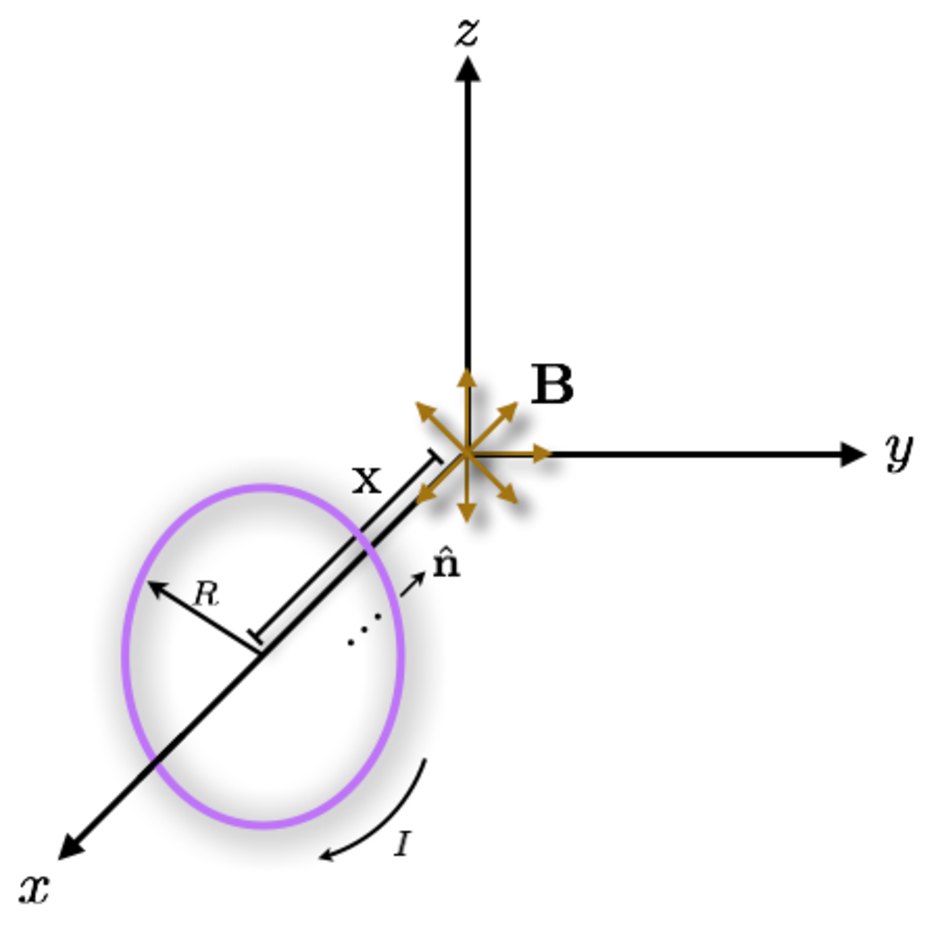
\includegraphics[width=0.4\textwidth]{fza-sobre-circuito-por-campoB}
%         \caption{\emph{Campo $\B$ radial que fluye desde el origen.}}\label{fza-sobre-circuito-por-campoB}
% \end{figure}\\
% \emph{Solución.}\\
% En el ejemplo (\ref{esp cn ind rad}) se encontró que la fuerza sobre una espira circular situada en el campo $\B=K\textbf{r}/r^3$ está dada por
% \begin{equation*}
%  \textbf{F}&=&IK\nabla\Omega.
% \end{equation*}
% Con
% \begin{equation}
% \Omega &=&-\int_S\frac{\hat{\textbf{r}}\cdot \textbf{i}\,da}{r^2},\nonumber\\
% &=&-\frac{\sin\theta\cos\varphi}{r^2}\int_S da,\nonumber\\
% &=&-\pi\,R^2\,\frac{\sin\theta\cos\varphi}{r^2}.
% \end{equation}
% Entonces
% \begin{equation}
% \nabla\Omega&=&\frac{\partial \Omega}{\partial r}\hat{\textbf{r}}+\frac{1}{r}\frac{\partial \Omega}{\partial \theta}\hat{\pmb{\theta}}+\frac{1}{r\sin\theta}\frac{\partial \Omega}{\partial \varphi}\hat{\pmb{\varphi}},\nonumber\\
% &=&\pi\,R^2\left( 2\frac{\sin\theta\cos\varphi}{r^3}\hat{\textbf{r}}-\frac{\cos\theta\cos\varphi}{r^3}\hat{\pmb{\theta}}+\frac{\sin\varphi}{r^3}\hat{\pmb{\varphi}}\right) .
% \end{equation}
% Finalmente, la fuerza ejercida sobre el circuito es
% \begin{equation}
% \textbf{F}&=&IK\frac{\pi\,R^2}{r^3}\left( 2\sin\theta\cos\varphi\,\hat{\textbf{r}}-\cos\theta\cos\varphi\,\hat{\pmb{\theta}}+\sin\varphi\,\hat{\pmb{\varphi}}\right).
% \end{equation}
% Con
% \begin{equation}
% r&=&\sqrt{x^2+R^2},\\
% \therefore \textbf{F}&=&\frac{IK\pi\,R^2}{(x^2+R^2)^{3/2}}\left( 2\sin\theta\cos\varphi\,\hat{\textbf{r}}-\cos\theta\cos\varphi\,\hat{\pmb{\theta}}+\sin\varphi\,\hat{\pmb{\varphi}}\right).
% \end{equation}
% \end{example}
%
